
\documentclass[12pt]{report}
\usepackage[utf8x]{inputenc}
\usepackage{graphicx}
\graphicspath{{images/}}
\usepackage{hyperref}
\usepackage{amsmath}
%\usepackage{chngpage}
%\usepackage{subfig}
%\usepackage{subfigure}
%\usepackage{float}
\usepackage[a4paper,tmargin=1.1in,bmargin=1.1in,lmargin=1.2in,rmargin=1in]{geometry}
%\usepackage{fancyhdr}
%\pagestyle{fancy}
\usepackage{enumitem}
\usepackage[algoruled,boxed,lined]{algorithm2e}
\usepackage{graphicx}
\usepackage{caption}
\usepackage[font={scriptsize}]{subcaption}
%\usepackage{subcaption}
\usepackage{array}
\usepackage{tikz}
\usetikzlibrary{shapes.geometric,arrows,positioning}
\tikzstyle{startstop}=[ellipse, minimum width=3cm, minimum height=0.6cm,text centered, draw=black, fill=white]
\tikzstyle{io}=[trapezium, trapezium left angle=70, trapezium right angle=110, minimum width=3cm, minimum height=0.6cm, text centered, draw=black, fill=white]
\tikzstyle{process}=[rectangle, minimum width=2cm, minimum height=0.6cm, text centered, draw=black, fill=white]
\tikzstyle{decision}=[diamond, aspect=2, minimum width=1.5cm, minimum height=0.8cm, text centered, draw=black, fill=white]
\tikzstyle{arrow} = [thick,->,>=stealth]
\tikzset{draw}

\usepackage{amsthm}
\usepackage{amsmath}
\usepackage{amssymb}

\theoremstyle{plain}
\newtheorem{thm}{Theorem}[chapter] % reset theorem numbering for each chapter
\newtheorem{theory}{Theorem}
\newtheorem{tlem}{Theorem}
\newtheorem{texmpl}{Theorem}
\theoremstyle{definition}
\newtheorem{defn}[thm]{Definition} % definition numbers are dependent on theorem numbers
\newtheorem{exmp}[texmpl]{Example} % same for example numbers
\newtheorem{lem}[tlem]{Lemma}

\newcommand\textbox[1]{%
  \parbox{.333\textwidth}{#1}%
}


\usepackage{titlesec}
 

\makeatletter
\def\@makechapterhead#1{%
  \vspace*{0\p@}%
  {\parindent \z@ \centering
    \normalfont
    \ifnum \c@secnumdepth >\m@ne
      \if@mainmatter
        \large \bfseries \@chapapp\space \thechapter
        \par\nobreak
        \vskip 20\p@
      \fi
    \fi
    \interlinepenalty\@M
    \LARGE \bfseries #1\par\nobreak
    \vskip 40\p@
  }}
\def\@schapter#1{\if@twocolumn
                   \@topnewpage[\@makeschapterhead{#1}]%
                 \else
                   \@makeschapterhead{#1}%
                   \@afterheading
                 \fi}
\def\@makeschapterhead#1{%
  \vspace*{0\p@}%
  {\parindent \z@ \centering
    \normalfont
    \interlinepenalty\@M
    \Large \bfseries  #1\par\nobreak
    \vskip 40\p@
  }}

\renewcommand\section{\@startsection {section}{1}{\z@}%
                                   {-6ex \@plus -1ex \@minus -.2ex}%
                                   {2.3ex \@plus.2ex}%
                                   {\normalfont\Large\bfseries}}

\renewcommand\subsection{\@startsection {subsection}{1}{\z@}%
                                   {-4ex \@plus -1ex \@minus -.2ex}%
                                   {2.3ex \@plus.2ex}%
                                   {\normalfont\large\bfseries}}

\makeatother

\begin{document}

\pagenumbering{roman}
\setcounter{page}{1}


% ############################################################################################################
%
% Title Page (only if you want to make it with LaTeX)
%

\begin{titlepage}
    \begin{center}
        \vspace*{1cm}
        
        \Large
        \textbf{Simultaneous image fusion and denoising based on multiscale transformation and sparse representation }
        
        
        \vspace{3.8cm}
        
        \textsl{
        Tahiatul Islam\\
        Roll: 1109056\\
        Supervisor: Dr. Sheikh Md. Rabiul Islam\\
        Associate Professor, ECE, KUET}
        
        \vspace{2.2cm}
        
        
\includegraphics[width=0.2\textwidth]{Logo_KUET.png}
        
        \vspace{1cm}
        \Large
        Department of Electronics \& Communication Engineering\\
        Khulna University of Engineering \& Technology\\
        Khulna, Bangladesh\\
        May, 2016
        
    \end{center}
\end{titlepage}

% ############################################################################################################



%\setlength{\parindent}{1em}
%%\setlength{\parskip}{1em}
%
%%\usepackage{titlesec}
%
%\titlespacing*{\section}
%{0pt}{5.5ex plus 1ex minus .2ex}{4.3ex plus .2ex}
%\titlespacing*{\subsection}
%{0pt}{5.5ex plus 1ex minus .2ex}{4.3ex plus .2ex}
%
%%\begin{document}
%


\addtocontents{toc}{~\hfill\textbf{Page}\par}

\chapter*{Acknowledgement}
\addcontentsline{toc}{chapter}{Acknowledgement}
%\renewcommand{\abstractname}{Acknowledgements}
%\begin{abstract}
With due homage and honor, I want to express my gratitude to Almighty.\\


\noindent I express my indebtedness to my dedicated supervisor Dr. sheikh Md. Rabiul Islam ( Associate Professor, Department of Electronics and Communication Engineering, KUET) for his necessary guidance, suggestions and encouragement to all phases of my work. I am also very grateful to our Departmental Head Dr. Md. Faruque Hossain (Professor,  Department of Electronics and Communication Engineering, KUET). I would also like to thank all the teachers who've been much helpful and encouraging in completion of our thesis work.\\

\noindent\textbox{\hfill}\textbox{\hfil \hfil}\textbox{\hfill \textbf{Author}}
%\end{abstract}

\chapter*{Abstract}
\addcontentsline{toc}{chapter}{Abstract}
%\renewcommand{\abstractname}{Abstract}
%\begin{abstract}
Image fusion is one of the currently active area in image processing society.The goal of image fusion is to increase the total information in a single image from number of source images.In previous year different method has been proposed in fusing image and each of them has its own pros \& cons. Multi-scale transform (MST) and sparse representation (SR) based method found most effective in image fusion.In my work i propose a method of image fusion which take the  advantage of both MST and SR in fusing image which also able to remove noise introduced in the source images.

%\end{abstract}


%\chapter*{Dedication}
%To mum and dad

\tableofcontents
%\addcontentsline{toc}{chapter}{Contents}
\listoffigures
\addcontentsline{toc}{chapter}{List of Figures}
\listoftables
\addcontentsline{toc}{chapter}{List of Tables}

%\setlength{\parskip}{1ex plus 0.5ex minus 0.2ex}

\chapter{Introduction}
\setcounter{page}{2}
\pagenumbering{arabic}
\section{Introduction}
 In recent years, image fusion has become an important issue in
image processing community. The target of image fusion is to generate a composite image by integrating the complementary information from multiple source images of the same scene. For
an image fusion system, the input source images can be acquired
from either different types of imaging sensors or a sensor whose
optical parameters can be changed, and the output called fused
image will be more suitable for human or machine perception than
any individual source image. Image fusion technique has been
widely employed in many applications such as computer vision,
surveillance, medical imaging, and remote sensing.
\hfill \break

 As shown in fig \ref{fig1} a,b shows the image whose center and boarder are blared respectively and c shows its fused image which contains the total information contain in source image a \& b.
\hfill \break

 I proposed a technique of image fusion based on MST and SR. In MST image is decomposed into band of low pass and high pass based on the decomposition method and sparse representation sparsely represent an image patch by a dictionary matrix. I combine above two method to take advantage in image fusion. Theoretical description of MST and SR will discuss in second chapter.

\begin{figure}[ht] 
  \begin{subfigure}[b]{0.33\linewidth}
    \centering
    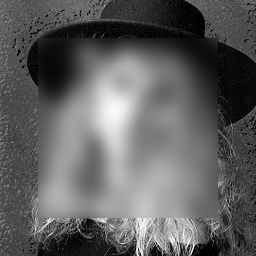
\includegraphics[width=0.5\linewidth]{1a}
    \caption{} 
    \label{1a} 
    \vspace{4ex}
  \end{subfigure}%%
  \begin{subfigure}[b]{0.33\linewidth}
    \centering
    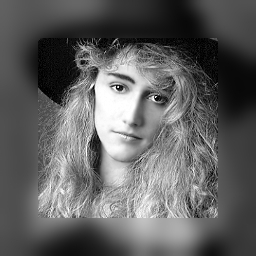
\includegraphics[width=0.5\linewidth]{1b}
    \caption{} 
    \label{1b} 
    \vspace{4ex}
  \end{subfigure}%%
  \begin{subfigure}[b]{0.33\linewidth}
    \centering
    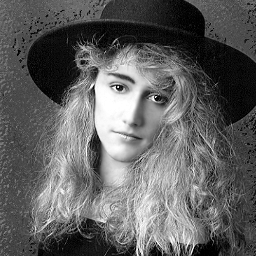
\includegraphics[width=0.5\linewidth]{1c} 
    \caption{} 
    \label{1c} 
    \vspace{4ex}
  \end{subfigure}%%
  
  \caption{(a),(b)Sensor image from two source.(c)Fused image of a,b.}
  \label{fig1} 
\end{figure}

\section{Motivation}
The major, recurrent theme throughout this work is my search for a good fusion model for image fusion of multifocous and natural
images. In addition, I seek a model for image fusion based on sparse representation that is capable of approximating the images with only fewer non zero coefficient. The hope is that I would find out a simple model that can fuse multiple images. Finally, the computation  time for the model would be small and fusing the images would be easy enough.

\section{Problem Statement}\label{sec:ProbStatement}
Being able to fuse multiple image is a very challenging task, but it could have great impact, for instance when taking image by digital camera it focus one object while another in different distance remain blurred or unfocused as shown in figure \ref{fig1.2} .My task is to fuse image from different source sensor and generate an image that is fully focus for every object at relative distance in the fused image.

\begin{figure}[h]
  \centering
  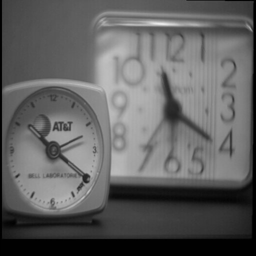
\includegraphics[width=0.5\linewidth]{1d.png}
  \label{fig2}
  \caption{Example of a multifocus image.}
\end{figure}


\section{Objectives}
% List items using bullets

\begin{itemize}
  \item First objective is to find efficient method to fuse images.
  \item Next objective is to remove any artifact produced by fusing transform coefficient. 
  \item To remove noise introduced in source image from fused image.
\end{itemize}




\chapter{Multi-Scale Transformation}
Multi-scale transform (MST) theories are the most popular tools
used in various image fusion scenarios such as multi-focus image fusion, visible-infrared image fusion, and multimodal medical image fusion. Classical MST-based fusion methods include pyramid-based ones like Laplacian pyramid (LP)\cite{2} 
 ratio of low-pass pyramid (RP)\cite{3} and gradient pyramid (GP)\cite{4},wavelet-based ones like discrete wavelet transform (DWT)\cite{5},stationary wavelet transform (SWT) \cite{6} and dual-tree complex wavelet transform (DTCWT) \cite{7}, and multi-scale geometric analysis (MGA)-based ones like curvelet transform (CVT)\cite{8} and nonsubsampled contourlet transform (NSCT) \cite{9}. 
\hfill \break 
In the following section i am going to discuss some of above featured transformation.

\section{Laplacian pyramid Transformation}

Pyramid, or pyramid representation, is a type of multi-scale signal representation developed by the computer vision, image processing and signal processing communities, in which a signal or an image is subject to repeated smoothing and subsampling. Pyramid representation is a predecessor to scale-space representation and multiresolution analysis.

\subsection{Pyramid Generation}
There are two main types of pyramids: lowpass and bandpass.
\hfill \break
A lowpass pyramid is made by smoothing the image with an appropriate smoothing filter and then subsampling the smoothed image, usually by a factor of 2 along each coordinate direction. The resulting image is then subjected to the same procedure, and the cycle is repeated multiple times. Each cycle of this process results in a smaller image with increased smoothing, but with decreased spatial sampling density (that is, decreased image resolution). If illustrated graphically, the entire multi-scale representation will look like a pyramid, with the original image on the bottom and each cycle's resulting smaller image stacked one atop the other. \hfill \break

A bandpass pyramid is made by forming the difference between images at adjacent levels in the pyramid and performing some kind of image interpolation between adjacent levels of resolution, to enable computation of pixelwise differences.
\hfill \break
A variety of different smoothing kernels have been proposed for generating pyramids

\begin{figure}[h]
  \centering
  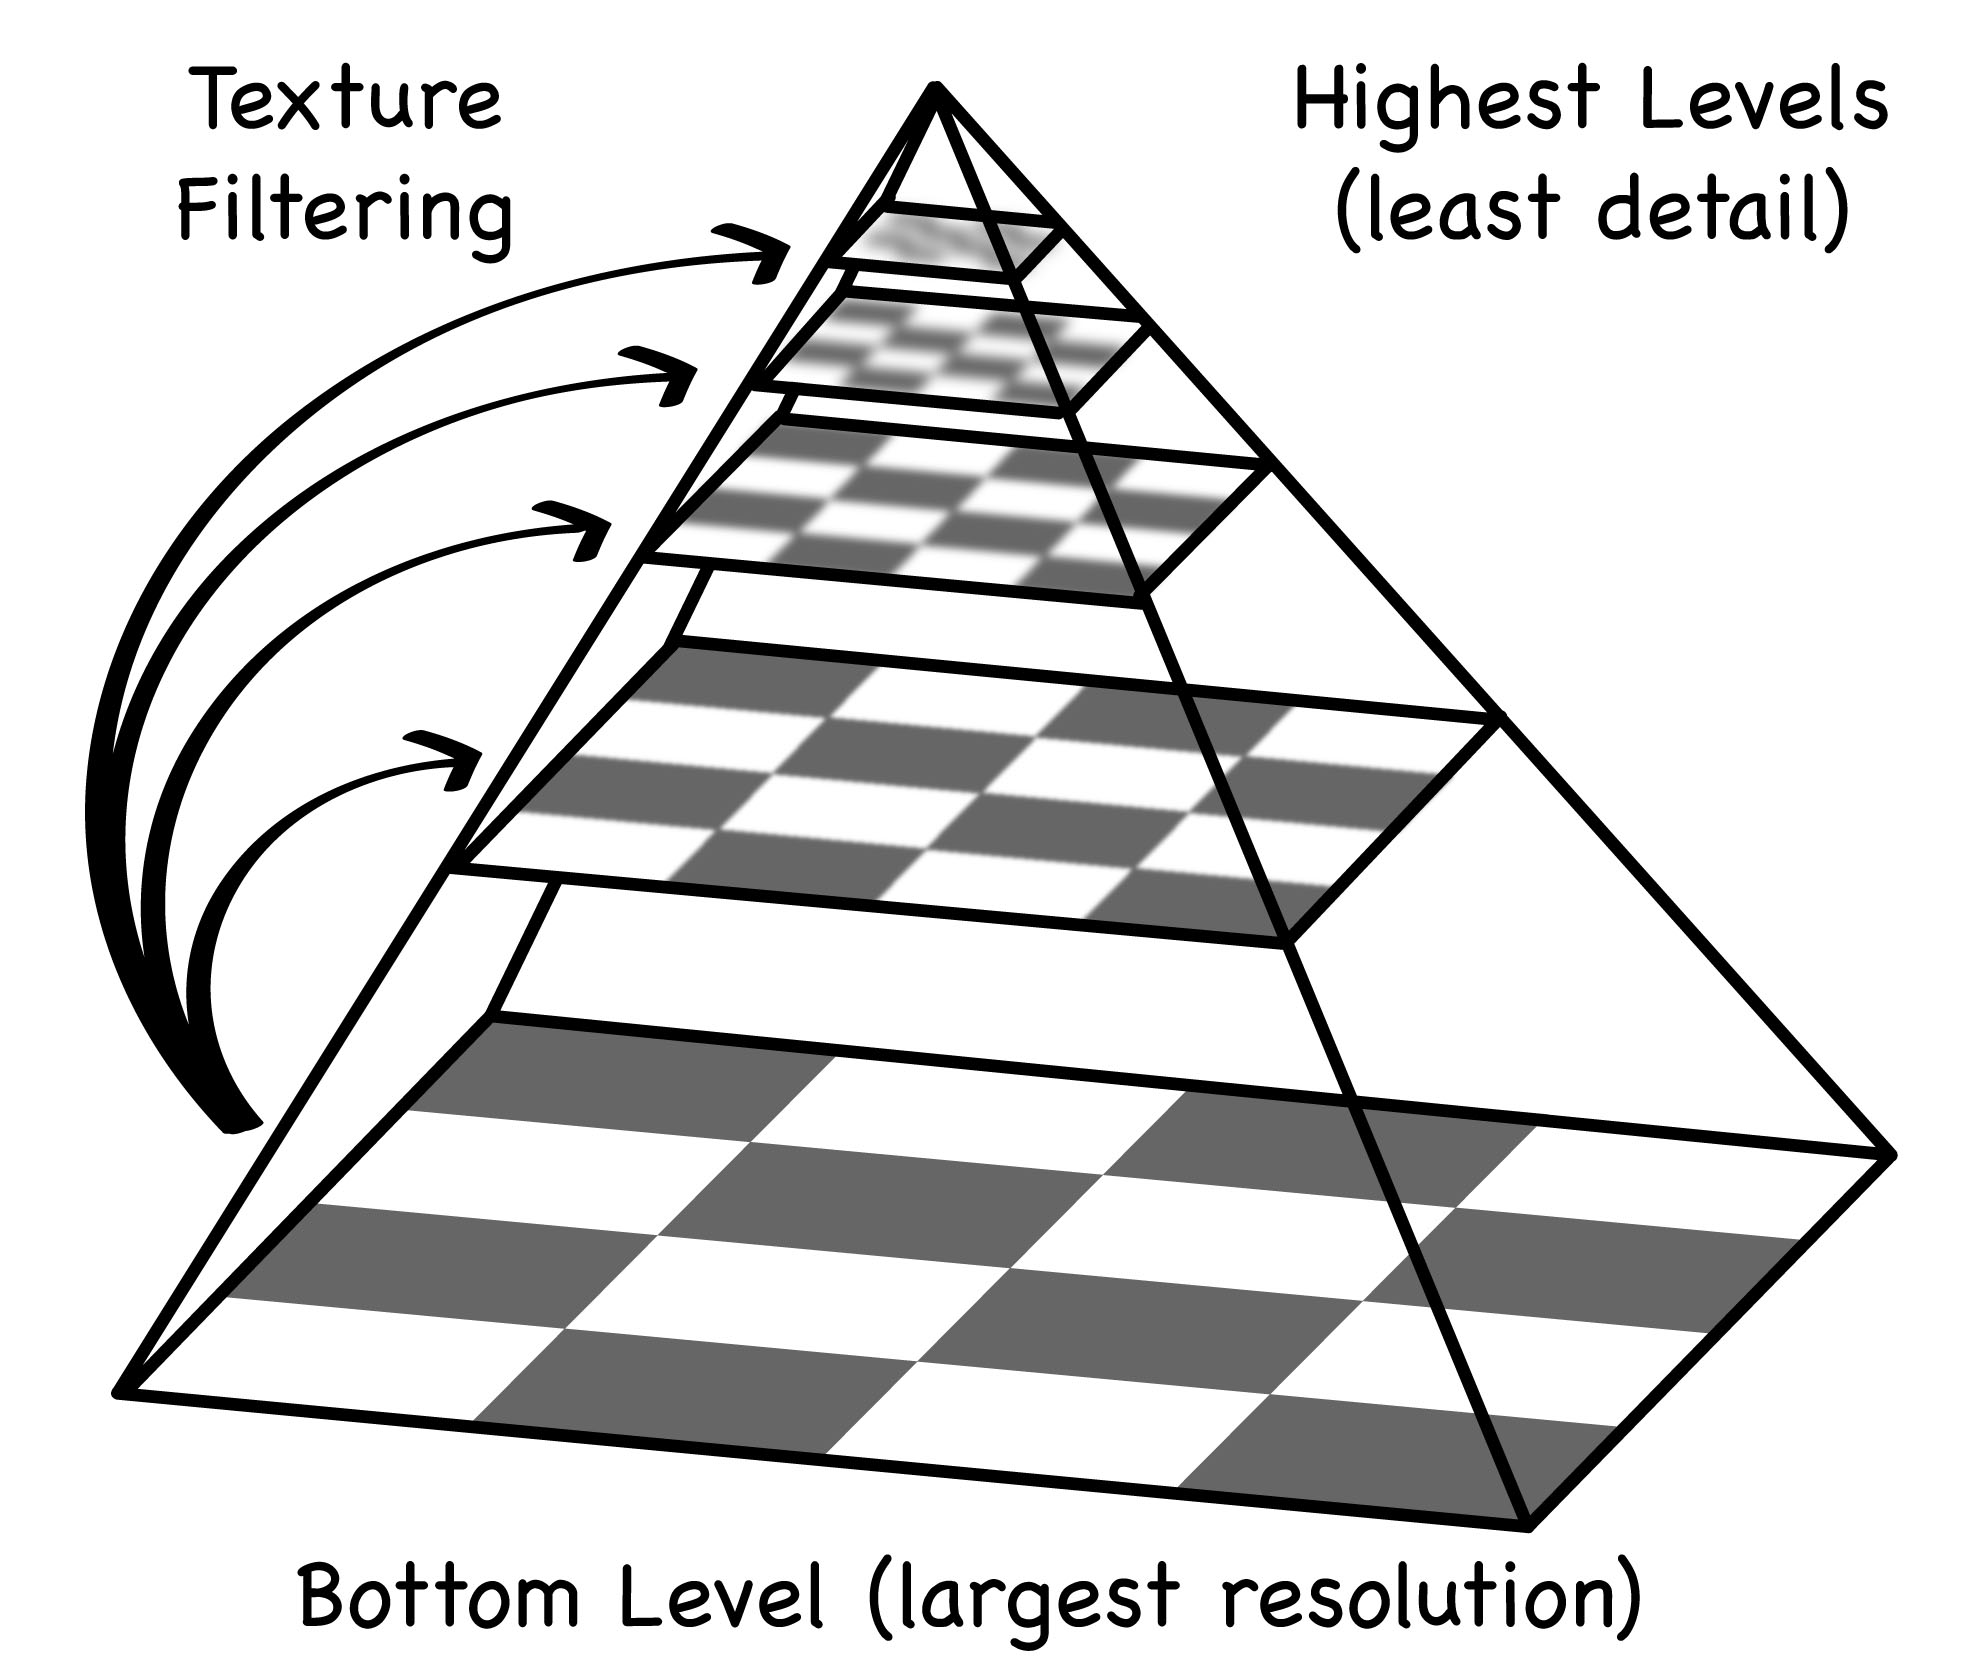
\includegraphics[width=0.5\linewidth]{2a.jpg}
  \label{fig2}
  \caption{Laplacial pyramid decomposition level}
\end{figure}

\section{Wavelet Transformation}
I start this section by introducing the specific concepts related to the wavelet transform, so that the reader
can understand the basic concepts associated with this transform. \hfill \break

 The analysis and synthesis procedures lead to the
pyramid-structured wavelet decomposition \cite{9}.The 1-D multiresolution wavelet decomposition can be easily extended to two dimensions by introducing separable 2-D scaling and wavelet functions as the tensor products of their 1-D complements. Hence, we obtain

\begin{equation}
    \begin{split}
    {\phi }_{LL}\left(x,y \right)=\phi \left(x \right)\phi \left(y \right)\vspace{1cm}
    {\psi }_{LH}\left(x,y \right)=\phi \left(x \right)\psi  \left(y \right)\\
	{\psi }_{HL}\left(x,y \right)=\psi \left(x \right)\phi  \left(y \right),\vspace{1cm}
	{\psi }_{HH}\left(x,y \right)=\psi \left(x \right)\psi  \left(y \right)  
    \end{split}
\end{equation}

The 2-D wavelet analysis operation consists in =ltering and
down-sampling horizontally using the 1-D lowpass =lterL(with impulse responses l(i)) and highpass =lterH(withimpulse responses h(j)) to each row in the imageI(x; y),producing the coeIcient matrices IL(x; y) and IH(x; y).
Vertically =ltering and down-sampling follows, using the lowpass and highpass =lters LandHto each column in IL(x; y) andIH(x; y) and produces four subimagesILL(x; y),ILH(x; y), IHL(x; y) and IHH(x; y) for one level of decomposition.ILL(x; y) is a smooth subimage corresponding to the low-frequency band of the MSD and can be considered as a smoothed and subsampled version of the original imageI(x; y), i.e. it represents the coarse approximation of I(x; y).ILH(x; y),IHL(x; y) andIHH(x; y) are detail subimages, which represent the horizontal, vertical and diagonal
directions of the imageI(x; y).
\begin{figure}[h]
  \centering
  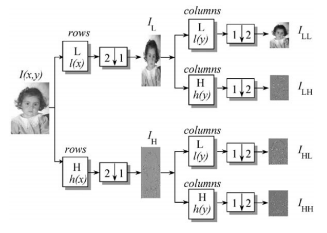
\includegraphics[width=0.5\linewidth]{2b.png}
  \label{fig2}
  \caption{ One stage of 2-D DWT multiresolution image decomposition
(forward wavelet analysis).}
\end{figure}

Fig \ref{fig2.2} depicts one stage in a multiresolution pyramid decomposition of the input imageI(x; y). In order to illustrate the
examples of this section, we have used the Haar wavelet
transform, although any other set of wavelets could be used.
Hence,L≡(1=√2)[1;1] and H≡(1=√2)[1;−1].The detailed 2-D pyramid decomposition algorithm, can be expressed as follows: Let I(x; y) be the original image of size M×N, l(i) the analysis lowpass coefficients of a specific wavelet basis, i =0;1,2......Nh−1, where Nl is the support length of the filter L, h(j) the analysis high pass coefficients of a specific wavelet basis,j=0,1....Nh−1, where Nh is the support length of the filter H. Then,

\begin{equation}
    \begin{split}
     {I}_{L}\left(x,y \right) &=\frac{1}{{N}_{l}} \sum_{i=0}^{{N}_{l}-1} I\left(i \right). I\left(\left(2x+i \right)modM,y \right),{I}_{H}\left(x,y \right)\\ &=\frac{1}{{N}_{h}} \sum_{j=0}^{{N}_{h}-1} h\left(j \right). I\left(\left(2x+j \right)modM,y \right) 
    \end{split}
\end{equation}
for x=0,1,2......M/2−1 and y=0,1,2......N−1

\begin{equation}
    \begin{split}
     {I}_{LL}\left(x,y \right) &=\frac{1}{{N}_{l}} \sum_{i=0}^{{N}_{l}-1} I\left(i \right). I\left(x,\left(2x+i \right)mod N \right),{I}_{LH}\left(x,y \right)
\\ &=\frac{1}{{N}_{h}} \sum_{j=0}^{{N}_{h}-1} h\left(j \right). I\left(x,\left(2y+j \right)mod N \right) 
    \end{split}
\end{equation}

\begin{equation}
    \begin{split}
    {I}_{HL}\left(x,y \right) &=\frac{1}{{N}_{l}} \sum_{i=0}^{{N}_{l}-1} I\left(i \right). {I}_{H}\left(x,\left(2y+i \right)mod N \right),{I}_{HH}\left(x,y \right) \\
\\ &=\frac{1}{{N}_{h}} \sum_{j=0}^{{N}_{h}-1} h\left(j \right). {I}_{H}\left(x,\left(2y+j \right)mod N \right)
    \end{split}
\end{equation}
for x=0,1,2......m/2-1 and y=0,1,2.....N/2-1 \\

The 2-D pyramid algorithm can iterate on the smooth subimage 
\({I}_{LL}\left(x,y \right)\) to obtain four coefficient matrices in the next decomposition level and so on. This is illustrated in Figs.\ref{fig2.3} and  which correspond to one-and two-level image decompositions, respectively.  \\ 

\begin{figure}[h]
  \centering
  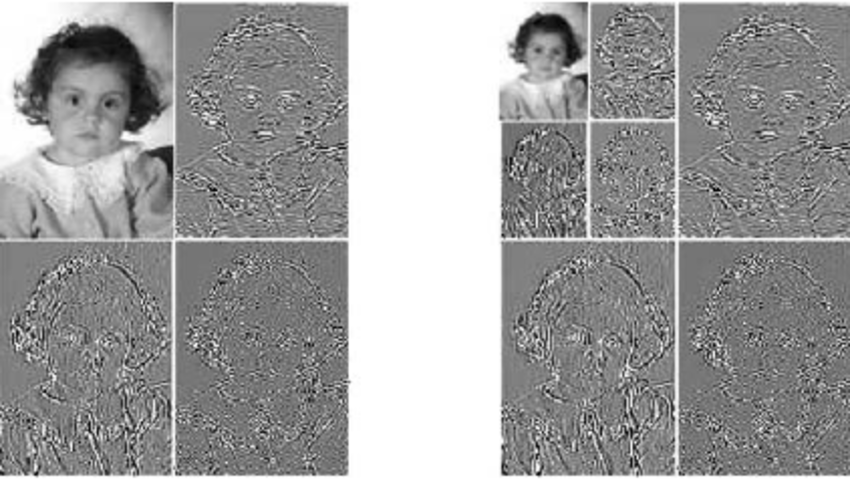
\includegraphics[width=0.5\linewidth]{2d.png}
  \label{fig2}
  \caption{ A representation of (a) one-level and (b) two-level image
decomposition.}
\end{figure}

Some wavelet-based applications do not require all coefficients, only the most relevant. So an additional procedure can be carried out to eliminate non-significant coefficient by thresholding, since these have a magnitude close to zero. After thresholding, only the desired coefficients remain.The threshold value can be chosen as \(T=\sigma\sqrt{2\log n/ \sqrt{n}}  \) in  where \(\sigma\)  is the standard deviation of the coefficients and n is the total size of samples. Another possibility is to fix T in order to replace a percentage of the coefficients with the
smallest magnitude to zero. Obviously, the cancellation of coefficients implies a loss of information. \\

The inverse 2-D wavelet transform can be implemented using a backward 2-D pyramid algorithm. The 2-D wavelet synthesis operation consists in up-sampling and filtering vertically using the 1-D synthesis lowpass filter
L(with impulse responses l(i)) and highpass filter H(with impulse
responses  h(j)) for each column in the subimage. Horizontal up-sampling and =ltering then follows, using the lowpass  Land highpass filter H, for each row of the reversed image. Fig. \ref{fig2.4} shows one stage in a wavelet reconstruction


\begin{figure}[h]
  \centering
  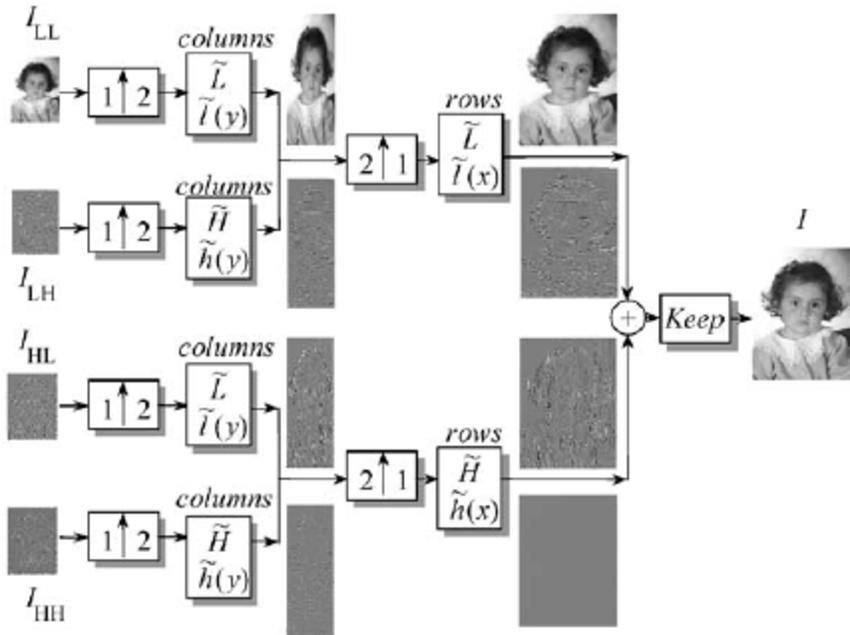
\includegraphics[width=0.5\linewidth]{2c.png}
  \label{fig2}
  \caption{One stage of 2-D DWT multiresolution image reconstruction
(backward wavelet synthesis).}
\end{figure}

\section{Fast Discrete Curvelet Transforms}
Despite considerable success, intense research in the last few years has shown that classical multiresolution ideas are far from being universally effective. Indeed, just as people recognized that
Fourier methods were not good for all purposes and consequently introduced new systems such as wavelets researchers have sought alternatives to wavelet analysis. In signal processing for example, one has to deal with the fact that interesting phenomena occur along curves or sheets, e.g.
edges in a two-dimensional image. While wavelets are certainly suitable for dealing with objects where the interesting phenomena, e.g. singularities, are associated with exceptional points, they
are ill-suited for detecting, organizing, or providing a compact representation of intermediate dimensional structures. Given the significance of such intermediate dimensional phenomena, there
has been a vigorous research effort to provide better adapted alternatives by combining ideas from geometry with ideas from traditional multiscale analysis 
\subsection{Why a discrete curvelet transform?}
Curvelets are interesting because they efficiently address very important problems where wavelet ideas are far from ideal. I give three examples:

\begin{itemize}
  \item Optimally sparse representation of objects with edges. Curvelets provide optimally sparse representations of objects which display curve-punctuated smoothness except for discontinuity along a general curve with bounded curvature. Such representations are nearly as sparse as if the object were not singular and turn out to be far more sparse than
the wavelet decomposition of the object.
  \item Optimally sparse representation of wave propagators. Curvelets may also be a very significant tool for the analysis and the computation of partial differential equations. For example, a remarkable property is that curvelets faithfully model the geometry of wave propagation. Indeed, the action of the wave-group on a curvelet is well approximated by simply translating the center of the curvelet along the Hamiltonian flows. A physical interpretation of this result is that curvelets may be viewed as coherent waveforms with enough frequency localization so that they behave like waves but at the same time, with enough spatial localization so that
they simultaneously behave like particles 
  \item Optimal image reconstruction in severely ill-posed problems. Curvelets also have special micro local features which make them especially adapted to certain reconstruction problems with missing data.
\end{itemize}

\subsection{Digital Curvelet Transform via Wrapping} 
The ‘wrapping’ approach assumes the same digital coronization as in Section 3.1, but makes a different, somewhat simpler choice of spatial grid to translate curvelets at each scale and angle. Instead of a tilted grid, we assume a regular rectangular grid and define ‘Cartesian’ curvelets in essentially the same way as before,
\begin{equation} \label{eq:2.5}
 c\left(j,l,k \right)=\int \hat{f}\left(\omega  \right){U}_{j}\left({S}^{-1}\omega  \right){e}_{i<b\omega> }
\end{equation}
The difficulty behind this approach is that, in the frequency plane, the window \({U}_{j,l}\left[n1,n2 \right] \) does not
fit in a rectangle of size \({2}^{j} {2}^{j/2}  \), aligned with the axes, in which the 2D IFFT could be applied to compute \ref{eq:2.5}. After discretization, the integral over \(\omega \) becomes a sum over n1, n2 which would extend beyond the bounds allowed by the 2-D IFFT. The resemblance of \ref{eq:2.5} with a standard 2D inverse FFT is in that respect only formal.hanged.\\

To understand why respecting rectangle sizes is a concern, we recall that \({U}_{j,l}\)  is supported in the parallelepipedal region
    
 \subsection{Architecture of the FDCT}   
 
 \begin{itemize}
  \item Apply the 2D FFT and obtain Fourier samples \( \hat{f}\left[n1,n2 \right],-n/2 \leq n1,n2 \leq n/2   \)
  \item  For each scale j and angle, form the product \({U}_{j,l} \hat{f}\left[n1,n2\right] \)
  \item  Wrap this product around the origin and obtain
  \item  Apply the inverse 2D FFT to each \({f}_{j,l} \), hence collecting the discrete coefficients \({c}^{D} \left(j,l,k\right) \)
\end{itemize}

\chapter{Sparse Representation of signal}
There are various methods available to implement image
fusion. Basically, these methods can be categorized into two
categories. The first category is the spatial domain-based methods, which directly fuse the source images into the intensity
values . The other category is the transformed domain-based methods, which fuse images with certain frequency or time frequency transforms Assuming that F(·) represents the “fusion operator,” the fusion methods in the spatial domain can be summarized as 
\begin{equation}
 {I}_{F}= F({I}_{1},{I}_{2} \dots{} {I}_{k})
\end{equation}
The simplest fusion method in spatial domain just takes
the pixel-by-pixel average of the source images. However, this
method often leads to undesirable side effects, such as reduced
contrast . If the source images are not completely registered,
then a single pixel-based method, such as spatial gradient (SG) based method, always results in artifacts in the fused
image. Therefore, some more reasonable methods were proposed to fuse source images with divided blocks or segmented
regions instead of single pixels. However, the blockbased fusion methods usually suffer from blockness in the fused image. For the region-based method, the source images are first segmented, and the obtained regions are then fused using their properties, such as spatial frequency or SG. The segmentation algorithms, usually complicated and time consuming, are of vital importance to the fusion quality.A more popular method that has been explored in recent years is by using multiscale transforms The transformed domain-based methods can be summarized as
\begin{equation}
{I}_{F}={T}^{-1}(F(T({I}_{1}),T({I}_{2})\dots{} T({I}_{j}))
\end{equation}
\hfill \break
 Because the fused image obtained by transform domain-based algorithms is globally created, a little change in a single coefficient of the fused image in the transformed domain may cause all the pixel values to change in spatial domain. As a result, undesirable artifacts may be produced in the fusion process using the multiresolution transform-based methods in some cases
Obviously, effectively and completely extracting the underlying information of the original images would make the fused image more accurate. Different from multiscale transformations, the sparse representation using an overcomplete dictionary that contains prototype signal atoms describes signals by sparse linear combinations of these atoms \cite{30-34} Two main characteristics of sparse representation are its overcompleteness and sparsity \cite{32}. Overcompleteness means that the number of basis atoms in the dictionary exceeds the number of image pixels or signal dimensions. The overcomplete dictionary that contains rich transform bases allows for more stable and meaningful representation of signals. Sparsity means that the coefficients corresponding to a signal are sparse, that is to say, only “a few descriptions” can describe or capture the significant structure information about the object of interest. Benefiting from its sparsity and overcompleteness, sparse representation theory has successfully been applied in many practical applications, including compression, denoising, feature extraction, classification, and so on \cite{32-34}. Recent studies have shown
that common image features can also be accurately described
by only a few coefficients or “a few descriptions” \cite{32}. 
In general, sparse representation is a global operation, in the sense that it is based on the gray-level content of an entire image. However, the image fusion quality depends on the accurate
representation of the local salient features of source images.
Therefore, a “sliding window” technique is adopted to achieve
better performance in capturing local salient features and keeping shift invariance.

\section{Sparse Representaion}
SR assumes that the signal \(Y \in {\textbf{R}}^{n}\) can be represented as a linear combination of given atoms.These atoms consist of an overcomplete dictionary \( D\in {\textbf{R}}^{n*k} 
, with n<<K \). The representation of y may either be exact \(D\theta=y \) or approximate \(|D\theta -y|\leq \epsilon \)  where 
\(\epsilon \) is the specified error.The details about dictionary D is discuss in following section. The vector \(\theta \in {\textbf{R}}^{k} \) is the coefficients of the signal. The coefficients with the fewest number of nonzero coefficients is certainly an appealing representation. Exact determination of the sparsest representation proves to be an non-deterministic polynomial time-hard problem.
Approximate solutions are considered instead. Basically, two approaches were proposed in previous researches. One approach is based on greedy algorithms such as Matching Pursuit (MP) and Orthogonal Matching Pursuit (OMP).All of these approaches are based on replacing the \({l}_{0} \) with the \( { l}_{p} \) -norm,where \({l}_{p}\) (0<p≤1) is defined as \({\parallel \theta \parallel}_{p}={\left(\sum_{i} { \mid {\theta }_{i}\mid}^{p} \right)}^{1/p}  \) \hfill \break

Let  \({Y}_{i} \in {\textbf{R}}_{n*L} \left(i=1,2,....\lambda \right) \) denote the L signals with dimension from the i’th sensor. We can represent \({Y}_{i}\) with common component \(\Theta c \in {\textbf{R}}^{K*L} \) and innovation component \(\Theta_{i}^{u} \in {\textbf{R}}^{k*L}  \)of sparse coefficient matrix,and noise \({n}_{i} \in {\textbf{R}}^{n*L} \).

\begin{equation}
{Y}_{i}={Y}^{c}+Y_{i}^{u}=D{\Theta}^{c}+D\Theta_{i}^{u}+{n}_{i}
\end{equation} 

\hfill \break The concatenated source images matrix can be represented sparsely by the concatenated coefficient matrix.
\begin{equation}\label{eq:3.2}
\begin{pmatrix}
{Y}_{1}  \\ 
{Y}_{2}\\ 
\vdots\\
{Y}_{\Lambda }
\end{pmatrix}=\begin{pmatrix}
D & D & 0 & \dots{} &0 \\ 
 D& 0 &D  & \dots{} & 0 \\ 
 \vdots{}& \vdots{}  &  \vdots{} & \vdots{}  & \vdots{} \\ 
 D& 0 & 0 & \dots{} & D 
\end{pmatrix}\begin{pmatrix}
{\Theta }^{c}\\ 
\Theta _{l}^{u}\\ 
 \vdots{}      \\ 
\Theta _{\Lambda }^{u}
\end{pmatrix}+\begin{pmatrix}
{n}_{1} \\ 
{n}_{2} \\ 
\vdots{} \\ 
{n}_{\Lambda }
\end{pmatrix}
\end{equation}
where \(D \in {\textbf{R}}^{n*K} \)is the overcomplete dictionary which shared by both the common component and the innovation
component. Let  \( Y= \begin{pmatrix}
{Y}_{1}  \\ 
{Y}_{2}\\ 
\vdots\\
{Y}_{\Lambda }
\end{pmatrix} \)   \\   \(D= \begin{pmatrix}
D & D & 0 & \dots{} &0 \\ 
 D& 0 &D  & \dots{} & 0 \\ 
 \vdots{}& \vdots{}  &  \vdots{} & \vdots{}  & \vdots{} \\ 
 D& 0 & 0 & \dots{} & D 
\end{pmatrix} \) , \(\Theta=\begin{pmatrix}
{\Theta }^{c}\\ 
\Theta _{l}^{u}\\ 
 \vdots{}      \\ 
\Theta _{\Lambda }^{u}
\end{pmatrix}  \), \(n=\begin{pmatrix}
{n}_{1} \\ 
{n}_{2} \\ 
\vdots{} \\ 
{n}_{\Lambda }
\end{pmatrix} \) \\

Then, Eq \ref{eq:3.2} can be rewritten as follows
\begin{equation}
Y=D\Theta+n
\end{equation}

A crucial step of the SR/JSR is the selection of such a dictionary D. Predefined basis functions like curvelets, bandlets, variants of wavelets, etc., can be used. However, the success of such prespecified dictionaries is often limited by their suitability in capturing the structure in the signals under consideration. For example, image contents have SR over wavelet dictionary, but audio signals are better represented by sinusoids.  A more generalized approach is to learn the basis vectors that are specialized in representing the signal in question.  Several algorithms available in the literature deal with this problem, such as the K-SVD algorithm, the method of optimal directions (MOD), and the
Majorization method \cite{9,12,13} The K-SVD algorithm is slow
due to the SR computation and SVD operation exists at
its each iteration.
 \hfill \break
 The MOD does the most natural thing as \(\hat{D}=arg {min}_{D}\parallel Y-DX\parallel _{F}^{2}=Y{X}^{T} {\left(X{X}^{T}\right)}^{-1}\) However, \(X{X}^{T}\) may not be always with full rank. The Majorization method, for the dictionary update, is slow due to using the“Landweber”update (which is a gradient descent update)
as described in Ref \cite{14} 

\section{SR for Image Fusion} 

Since the sparse representation globally handles an image,
it cannot directly be used with image fusion, which depends
on the local information of source images. In my method, we
divide the source images into small patches and use the fixed
dictionary D with small size to solve this problem. In addition,
a sliding window technique is adopted to make the sparse
representation shift invariant, which is of great importance to
image fusion.
\hfill \break
We assume that source image I is divided into many image
patches. As shown in Fig.\ref{fig3.1}, to facilitate the analysis, the $\big(j^{th} \big) $ patch with size $ n×n $ is lexicographically ordered as a vector \({V}^{j}\). Then, \({V}^{j}\) can be expressed as
\begin{equation}
{V}^{j}=\sum_{t=1}^{T} {S}^{j} \left(t\right){d}_{t}
\end{equation}

where \({d}_{t}\) is an atom from a given overcomplete dictionary, and \(D\left[[{d}_{1} \dots{} {d}_{t} \dots{} {d}_{T} \right]\), which contains T atoms.\({S}_{j} = [{s}_{j}\left(1\right) \dots{} {s}_{j}\left( t\right) \dots{} {s}_{j}(T)]\)
 is the sparse representation

Assume that the vectors responding to all the patches in
image I are constituted into one matrix V. Then, Vcan be
expressed as 
\begin{equation}\label{eq:3.5}
D= \left[{d}_{1},{d}_{2} \dots{} {d}_{T}\right] \begin{pmatrix}
{S}^{1}(1) & {S}^{2}(1) & \dots{} & {S}^{j}(1) \\ 
 {S}^{1}(2)& {S}^{2}(2) & \dots{}  & {S}^{j}(2) \\ 
 \vdots{}& \vdots{}  &  \vdots{} & \vdots{}   \\ 
 {S}^{1}(T)& {S}^{2}(T) &  \dots{} & {S}^{j}(T) 
\end{pmatrix}
\end{equation}
where J is the number of image patches. Let \(S=[{s}^{1},{s}^{2},....,{s}^{j}]\). Then, eq. \ref{eq:3.5} can be expressed as 
\begin{equation}
V=DS
\end{equation}

\begin{figure}[h]
  \centering
  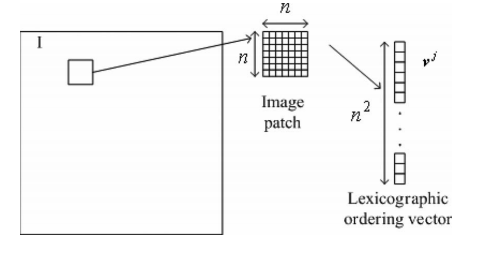
\includegraphics[width=0.5\linewidth]{3a.png}
  \label{fig3.1}
  \caption{Selected image patch and its lexicographic ordering vector.}
\end{figure}

\begin{figure}[h]
  \centering
  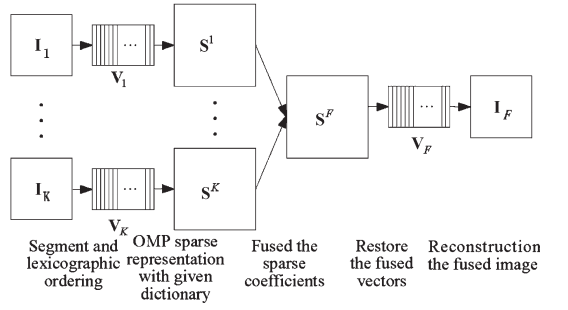
\includegraphics[width=0.5\linewidth]{3b.png}
  \label{figsr}
  \caption{Schematic diagram of the proposed SR-based fusion method.}
\end{figure}

where S is a sparse matrix.

\section{Training Dataset}
The Dictionary D is learnt from a database consisting of different type of multifocus images like medical image, infrared images, etc.
\hfill \break

I first randomly assign value in dictionary D of size \(64*256 \) from the image patches of training dataset image then i do sparse coding to get the sparse matrix of signal then i run K-SVD algorithm to update the dictionary.
\hfill \break

The training data consists of 100,000 \(8*8\)
patches, which are randomly sampled from a database of 40
high-quality natural images. The dictionary size is set to 256 and
the iteration number of K-SVD is fixed to 180.









\chapter{Image Denoising}
\section{Introduction}
In many applications, image denoising is used to produce good estimates of the original image from noisy observations.   The restored image should contain less noise than the observations while still keep sharp transitions (i.e. edges). \\


Wavelet transform, due to its excellent localization property, has rapidly become an indispensable signal and image processing tool for a variety of applications, including 
compression and denoising \cite{21,22,23}.   Wavelet denoising attempts to remove the noise present in the signal while preserving the signal characteristics, regardless of its 
frequency content.   It involves three steps:a linear forward wavelet transform, nonlinear  thresholding step and a linear inverse wavelet transform.\\

Wavelet thresholding (first proposed by Donoho \cite{21,22,23}) is a signal estimation technique that exploits the capabilities of wavelet transform for signal denoising.   It removes noise  by killing coefficients that are insignificant relative to some threshold, and turns out to be simple and effective, depends heavily on the choice of a thresholding parameter and the choice of this threshold determines, to a great extent the efficiency of denoising. Researchers have developed various techniques for choosing denoising parameters and so far there is no "best" universal threshold determination technique. \\

In my method i decompose the image by MST used in the transformation then apply BayesShrink soft thresolding to remove the insignificant coefficient the The aim of this project was to study various thresholding techniques such as  SureShrink \cite{21}, VisuShrink \cite{23} and BayesShrink \cite{22} and determine the best one for image 
denoising.

\section{Hard and soft thresholding}

Hard and soft thresholding with threshold ¸ are defined as follows: \\
The hard thresholding operator is defined as:
\begin{equation}
    \begin{split}
  D(U,T)=
\begin{cases}
 T& \text{ if } U>T \\
 0 &\text{ if } otherwise  
\end{cases}
    \end{split}
\end{equation}
The soft thresholding operator on the other hand is defined as:
\begin{equation}
D(U,T)=sgn\left(U \right)\max \left(0,\mid U \mid-\lambda  \right)
\end{equation}

\begin{figure}[h!]
  \centering
  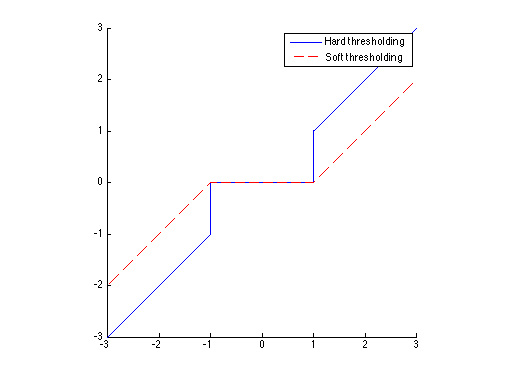
\includegraphics[width=.8\textwidth]{4a.png}
  \caption{soft and hard thresholding} \label{tsr}
\end{figure}

Hard threshold is a “keep orkill” procedure and is moreintuitively appealing. The transfer function of the same is shown in Fig \ref{tsr}. The alternative, soft thresholding  
(whose transfer function is also shown in Fig \ref{tsr}), shrinks coefficients above the threshold in absolute value. While at first sight hard thresholding may seem to be natural, the continuity of soft thresholding has some advantages. It makes algorithms  mathematically more tractable \cite{23}. Moreover, hard thresholding does not even work with some algorithms such as the GCV procedure . Sometimes, pure noise 
coefficients may pass the hard threshold and appear as annoying ’blips’ in the output. Soft thesholding shrinks these false structures. 

\section{Image denoising using thresholding}
As one may observe, threshold selection isan important question when denoising. A small threshold may yield a result close to the input, but the result may still be noisy.   A 
large threshold on the other hand, producesa signal with a large number of zero coefficients.   This leads to a smooth signal.Paying too much attention to smoothness, however, destroys details and in image processing may cause blur and artifacts. \hfill \break
The problem boils down to finding an optimal threshold such that the mean squared error  between the signal and its estimate is minimized. The wavelet decomposition of an 
image is done as follows: In the first level of decomposition, the image is split into 4 subbands, namely the HH, HL, LH and LL subbands. The HH subband gives the diagonal details of the image; the HL subband gives the horizontal features while the LH subband represents the vertical structures. The LL subband is the low resolution residual consisting of low frequency components and it is this subband which is further  split at higher levels of decomposition.  The different methods for denoising investigate differ only in the selection of the threshold. \hfill \break
I use the above perception of denoising for every MST i used.
So the basic procedure is 
\begin{itemize}
\item Calculate the MST coefficient of the image
\item Threshold the coefficient
\item Inverse transform the coefficient to get the denoised image.
\end{itemize}

\subsection{BayesShrink}
BayesShrink is an adaptive data-driven threshold for image denoising via wavelet soft-thresholding.The threshold is driven in a Bayesian framework, and we assume 
generalized Gaussian distribution (GGD) for the wavelet coefficients in each detail subband and try to find the threshold T which minimizes the Bayesian Risk.It is  found that BayesShrink performs better than SureShrink in terms of MSE. The reconstruction using BayesShrink is  smoother and more visually appealing than one obtained using SureShrink. 
\hfill \break

The BayesShrink threshold is given by :
\begin{equation}\label{bayest}
\hat{T}\left(\hat{{\sigma }_{I}} \right)=\frac{\hat{{\sigma }_{n}}}{\hat{{\sigma }_{I}}}
\end{equation}

where \({\sigma}_{n}\) and \({\sigma}_{I}\) are noise and signal standard deviations respectively.To estimate the noise variance\({\sigma}_{n}^{2}\) from the subband details, the median estimator is used on the 1-D subband coefficients:

\begin{equation}
\hat{{\sigma }_{n}}=median\left(\mid Details  \mid  \right)/0.6745
\end{equation}
the observed signal S is considered to be \( S=I+n\) and signal (I) and noise (n)are assumed to be independent.Therefore, 
\begin{equation}
\sigma _{S}^{2}=\sigma_{I}^{2}+\sigma_{n}^{2}
\end{equation}
where \(\sigma_{S}^{2} \)is the variance of the observed signal. So \(\sigma_{I}^{2}\)is estimated by:
\begin{equation}
\hat{\sigma_{I}}=\sqrt{\max\left(\left(\hat{{\sigma}_{S}^{2}}-\hat{\sigma _{n}^{2}} \right),0 \right)}
\end{equation}










\chapter{Propsed method}
\section{Proposed fusion framework}
the schematic diagram of the proposed fusion framework is shown in Fig\ref{fig:method} . In the Fig\ref{fig:method} only the fusion of two source images is considered while the proposed framework can be straightforwardly extended to fuse more than two images. The detailed fusion scheme contains the following four steps  \hfill \break


\begin{enumerate}
   \item \textbf{MST decompositon:}   Perform a specific MST on the two source images \( \left\{    {I}_{A},{I}_{B}\right\}  \)to obtain their low-pass bands \(\left\{{L}_{A},{L}_{B}\right\} \) and high-pass bands which are uniformly denoted as
 \(\left\{{H}_{A},{H}_{B}\right \} \)
 \item \textbf{Thresholding:} Perform thresholding as obtain in eq.\ref{bayest} on the low pass and high pass band to remove the unnecessary coefficient from the decomposition.  
    
	\item  \textbf{Low-pass fusion:} 	    
   \begin{itemize}
     \item Apply the sliding window technique to divide \( \left\{ {I}_{A},{I}_{B}\right\}  \)  into image patches of size \(\sqrt{n}\times\sqrt{n}\) from upper left to lower
right with a step length of s pixels. Suppose that there are
T patches denoted as \( \{{P}_{A}^{i}\}_{i=1}^{T}   \)
and  \( \{{P}_{B}^{i}\}_{i=1}^{T} \) in \({L}_{A}\) and \({L}_{B}\) respectively
respectively
     \item For each position i,rearrange \(\{P_{A}^{i},P_{B}^{i} \} \) into column vectors rearrange \(\{ \hat{V}_{A}^{i},\hat{V}_{B}^{i} \} \) by \begin{equation}
     \hat{V}_{A}^{i}=V_{A}^{i}-\bar{V}_{A}^{i}.1
     \end{equation}
     \begin{equation}
     \hat{V}_{B}^{i}=V_{B}^{i}-\bar{V}_{B}^{i}.1
     \end{equation}
     whre 1 denotes an all=one valued \(n \times 1 \) vector \(\bar{V}_{A}^{i}\) and \(\bar{V}_{B}^{i}\) are mean values of all the elements in \({V}_{A}^{i}\) and \({V}_{B}^{i}\) respectively.
     \item Calculate the sparse coefficient vectors \( \{\alpha_{A}^{i},\alpha_{B}^{i} \} \) of \(\{ \hat{V}_{A}^{i},\hat{V}_{B}^{i} \}\)using the orthogonal matching pursuit (OMP) algorithm \cite{24} by
     \begin{equation}
    \alpha _{A}^{i}=\arg \min \parallel \alpha \parallel _{0}   st \parallel \hat{V}_{A}^{i}-D\alpha \parallel_{2} < \epsilon     
\end{equation}      
\begin{equation} \label{eq:6}
\alpha _{B}^{i}=\arg \min \parallel \alpha \parallel _{0}   st \parallel \hat{V}_{B}^{i}-D\alpha \parallel_{2} < \epsilon
\end{equation}
where \textbf{D} is the learned dictionary.
\item Merge \( \alpha_{A}^{i} and \alpha_{B}^{i} \) with the "max-L1" rule to obtain the fused sparse vector
\begin{equation}
\alpha_{F}^{i}=
\begin{cases}
\alpha_{A}^{i} & \text{ if } \parallel \alpha_{A}^{i} \parallel_1 > \parallel \alpha_{B}^{i} \parallel_1\\ 
\alpha_{B}^{i} & \text{ otherwise } 
\end{cases}
\end{equation}
The fused result of \(V_{A}^{i} and V_{B}^{i}\) is calculated by \begin{equation}
V_{F}^{i}=D\alpha_{F}^{i}+\bar{V}_{F}^{i}.1
\end{equation}
where the merged mean value \(\bar{V}_{F}^{i}\) is obtained by 
\begin{equation} \label{eq:8}
\bar{V}_{F}^{i}=
\begin{cases}
\bar{V}_{A}^{i} & \text{ if }  \alpha_{F}^{i} =  \alpha_{B}^{i} \\ 
\bar{V}_{B}^{i} & \text{ otherwise } 
\end{cases}
\end{equation}
\item  Iterate the above process for all the source image patches in \(\{P_{A}^{i} \}_{i=1}^{T} \) and \(\{P_{B}^{i} \}_{i=1}^{T} \)to obtain all the fused vectors \(\{V_{F}^{i} \}_{i=1}^{T} \). Let \(L_{f}\) denotes the low-pass fused result. For each \(V_{F}^{i}\)reshape it into a patch \( p_{F}^{i}\)and then plug  \( p_{F}^{i}\)Finto its original position in \(L_{F}\).As patches are overlapped, each pixel’s value in \(L_{F}\) is averaged over its accumulation times
  \end{itemize}
   
   \item \textbf{High-pass fusion :} Merge \(H_{A} and H_{B}\)to obtain \(H_{F}\) with the popular "max-absolute"
rule using the absolute value of each coefficient as the activity level measurement. Then, apply the consistency verification scheme  to ensure that a fused coefficient does not originate from a different source image from most of its
neighbors. This can be implemented via a small majority filter

\item \textbf{MST reconstruction} Perform the corresponding inverse MST over \(L_{F} and H_{F}\) to reconstruct the final fused image \(I_{F}\)
\end{enumerate}

\begin{figure}[h!]
  \centering
  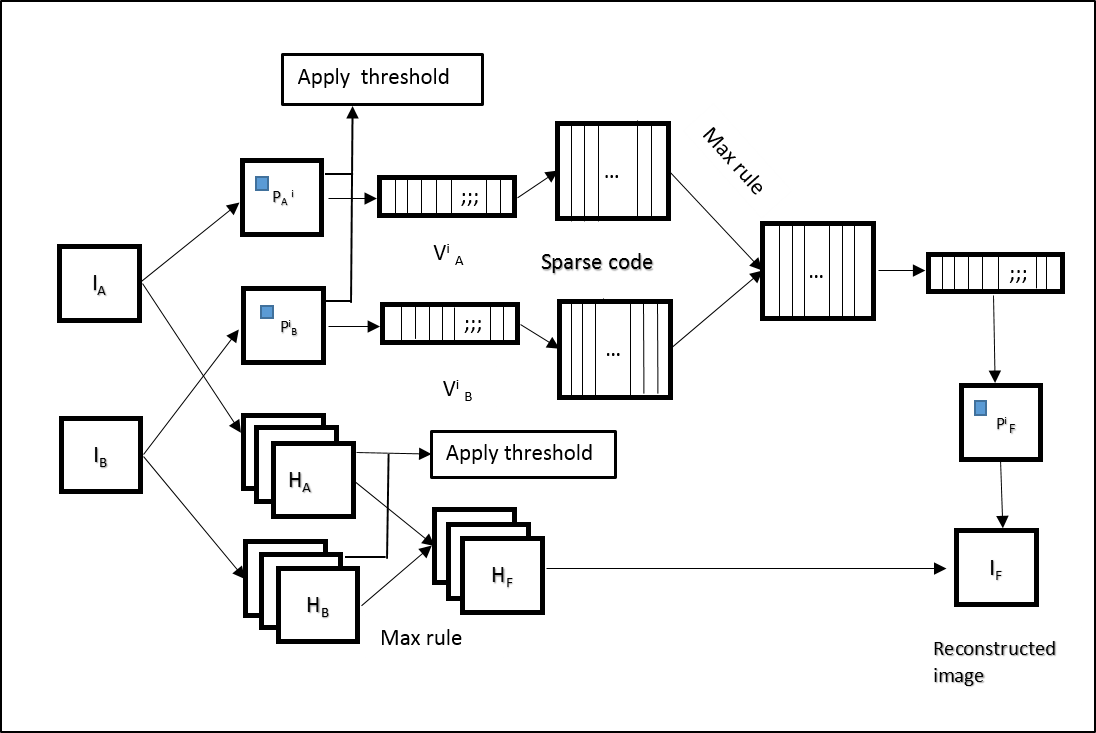
\includegraphics[width=.8\textwidth]{method.png}
  \caption{The schematic diagram of the proposed fusion framework} \label{fig:method}
\end{figure}

\section{Advantage over the MST based methods}
For the conventional MST-based image fusion methods (the
high-pass bands are merged with the "max-absolute" rule while the low-pass bands are fused using the "averaging" rule), there are two main drawbacks as follows \hfill \break

The first one is the loss of contrast. Since most energy of an
image is contained in the low-pass band (even though the decomposition level is set to 4 according to the analysis , the "averaging" fusion rule tends to lose some energy in the source images. For multi-focus image fusion, this phenomenon is not obvious because the source images are captured from the same type of sensors. However, for the fusion of multimodal images such as visible-infrared and medical images, the fused results of the MST-based methods are often in low contrast. This is mainly because different imaging modalities reflect different physical attributes, so a same region in different source images may have different brightness. For example,Fig. \ref{fig:advntg} shows a pair of computed tomography (CT) and magnetic resonance (MR) images. It can be seen that the CT image mainly focuses on dense structures like bones, while the MR image provides excellent soft-tissue details. When the "averaging" rule is used for low-pass fusion, the energy contained in those regions will be lost to a large extent.
As a result, the contrast of those regions in the fused image will decrease a lot after MST reconstruction \hfill \break

The second one is the difficulty in selecting the MST decomposition level. On one hand, to ensure enough spatial details can be extracted from the source images, the decomposition level cannot be too small such as 1 or 2. On the other hand, Li et al.\cite{25} experimentally verified that when the decomposition level is too large, one coefficient in the low-pass band have an impact on a large set of pixels in the fused image, so an error in the low-pass band (mainly caused by noise or mis-registration between the source images) will lead to serious artificial effects. Moreover, when the decomposition level becomes larger, the quality of high-pass fusion is also more sensitive to noise and mis-registration. Therefore, when the source images are not precisely registered, the decomposition level cannot be too large. Particularly, for multi-focus image fusion, due to the different imaging parameters (e.g. focal length) for multiple source images, the locations of object edges in different
source images are often not exactly the same for their different sharpness. A typical example is shown in Fig.\ref{advntg} Between the two source images, both the borders and numbers of the two clocks in the scene have different sharpness, so it is practically impossible to make an accurate registration. Thus, a compromise on decomposition level should be made for the consideration of extracting enough spatial details and being robust to mis-registration.\hfill \break

As a smart blending approach, the SR-based image fusion
scheme is combined into the MST-based fusion methods to
overcome the above two defects. In the proposed framework, the
SR-based scheme is employed to fuse the MST low-pass bands.In
Section2, after applying the "max-L1" rule in Eq.\ref{eq:6}, we transfer the energy in source images to the fused image by Eq.\ref{eq:8}.Therefore, the contrast in the fused image is improved. For the second defect, by extracting spatial details in low-pass band with the SR-based fusion scheme, the decomposition level can be set less than 4 for multi-focus image fusion to make the method more robust to mis-registration. Thus, the difficulty in determining decomposition level can be well solved.

\section{Advantages over the SR-based method}
The conventional SR-based image fusion method[14] mainly
has the following three defects.\hfill \break

The first one is the fine details in source images like textures and edges tend to be smoothed for the following two reasons. First, the signal representation ability of the dictionary may be not sufficient for fine details, which means that the reconstruction result is not approximate to the input signal. As we know, the representation ability of the over-completed dictionary relies much on the number of atoms in it, but a dictionary with a large size will directly increase the computational cost. More importantly, the study in[22]shows that a highly redundant dictionary may lead to potential visual artifacts in the reconstruction result, especially
when the input signal is corrupted by noise. Thus, a compromise on dictionary size is usually required. A typical example is that the dictionary size is 256 when the input signal is 64 dimensional \(8 \times 8\). Second, the usage of sliding window technique may also cause smoothness. The step length of the sliding window is usually set to 1 when fusing images directly in spatial domain to avoid blocking effects. However, when the adjacent patches are greatly overlapped, some details in the fused image will be smoothed. \hfill \break

The second one is the "max-L1" rule may cause spatial inconsistency in the fused image when the source images are captured by different imaging modalities. As mentioned before, for multimodal image fusion, a region may be very bright in one source image while very dark in another, but the region in both of them may be very "flat" with few fine details. Note that although a region in each of two source images is visually "flat", there still exists little difference between the two source images in terms of variance, and the difference is usually consistent over all the patches in that region. That is to say, if one patch in the region of source image A
has a larger variance than the corresponding patch in source image B, then most of the other patches in that region of source image A also tend to have larger variances than the corresponding patches in source image B. However, since the difference is very tiny, the "max-L1" fusion rule will become very sensitive to the random noise in spatial domain because a small change of value at a pixel may influence the fusion result of several patches. As a result, the fused patches in that region may originate from different source images, which will lead to spatial inconsistency in the fused image. Since the SR-based method handles patches in spatial domain, the
impact of high-frequency noise is considerable. \hfill \break

The third one is the low computational efficiency. Since the sliding window’s step length should be small enough, the sparse coding technique is performed on a large number of image patches. For instance, when the patch size is \(8\times8 \) and the step length is set to 1, there are 62001 patches to be processed for a source image of size \(256 \times256\) . In this case, it usually takes several minutes to fuse two source images with the SR-based method \hfill \break

The proposed fusion framework can effectively overcome the
above three defects of the SR-based method. In our fusion framework, the high-frequency spatial information is separated by performing MST and extracted by the "max-absolute" rule.
Meanwhile, the representation ability of the dictionary is enough to satisfy the reconstruction accuracy for low-frequency components. Furthermore, we will show in the next section that the sliding window’s step length in low-pass bands can be set larger than that in spatial domain. Therefore, the inclination of SR-based method to smooth fine details can be prevented. For the second defect, without high-frequency details, the random noise can be effectively eliminated, so the probability that the patches in a "flat" 
region originate from different source images will decrease to a large extent, leading to better spatial consistency. Finally, the computational efficiency can also be improved by the proposed framework because the number of patches required to be processed with the sparse coding technique is greatly reduced. For one thing, the step length can be set larger. For another, the low-pass bands of many MSTs such as LP and DWT have smaller size relative to the original image. \\ \\ 

\begin{figure}[ht] 
  \begin{subfigure}[b]{0.25\linewidth}
    \centering
    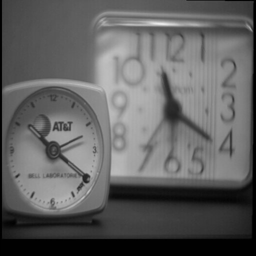
\includegraphics[width=0.5\linewidth]{5a.png}
    \caption{} 
    \label{1a} 
    \vspace{4ex}
  \end{subfigure}%%
  \begin{subfigure}[b]{0.25\linewidth}
    \centering
    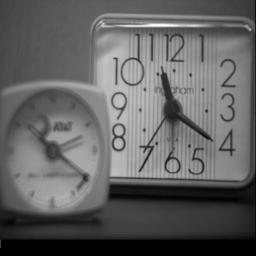
\includegraphics[width=0.5\linewidth]{5b.png}
    \caption{} 
    \label{1b} 
    \vspace{4ex}
  \end{subfigure}%%
  \begin{subfigure}[b]{0.25\linewidth}
    \centering
    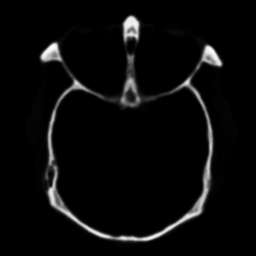
\includegraphics[width=0.5\linewidth]{5c.png} 
    \caption{} 
    \label{1c} 
    \vspace{4ex}
  \end{subfigure}%%
  \begin{subfigure}[b]{0.25\linewidth}
    \centering
    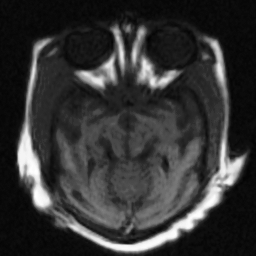
\includegraphics[width=0.5\linewidth]{5d.png}
    \caption{} 
    \label{1d} 
    \vspace{4ex}
  \end{subfigure}%%
  \caption{Two pairs of source images. (a,b)multi-focus images , and (c,d)  Medical images .}
  \label{advntg} 
\end{figure}



\chapter{Experiment setup and fusion evaluation metrics}
\section{Source images}
As shown in Fig.\ref{fig:6.1}, source images grouped into three categories are employed to verify the effectiveness of the proposed fusion framework. Among them, there are  multi-focus images Figs.\ref{fig:6.1},visible-infrared images Fig. \ref{fig:6.1}
and  medical images \ref{fig:6.1}. For each pair, the two
source images are assumed to be pre-registered in our study.

\begin{figure}[h!]
  \centering
  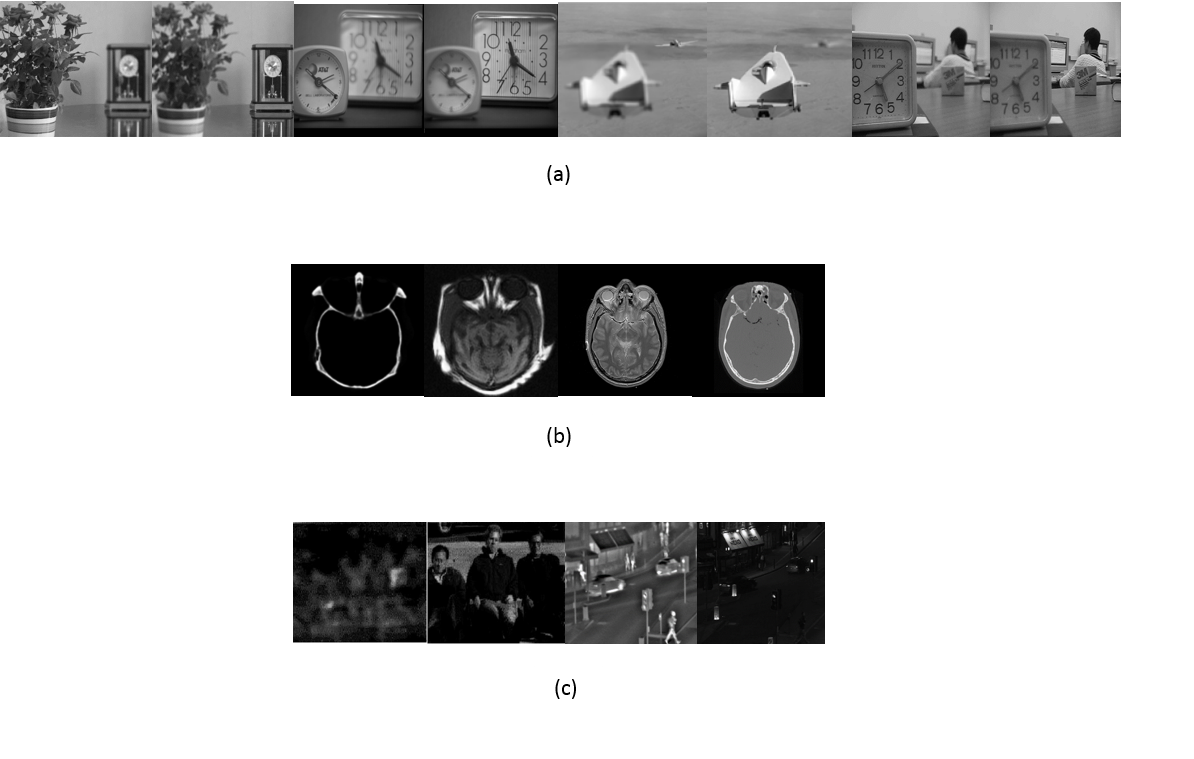
\includegraphics[width=1\textwidth]{sources.png}
  \caption{The source images used in our experiments. (a) Multi-focus images,(b)medical images   and (c) visible-infrared images} \label{fig:6.1}
\end{figure}

\section{Objective evaluation metrics}
It is not an easy task to quantitatively evaluate the quality of a fused image since the reference image (ground truth) does not
exist in practice. In recent years, many fusion metrics have been
proposed, but none of them is universally believed to be always
more reasonable than others for various fusion scenarios. Thus, it is usually necessary to apply several metrics to make a comprehensive evaluation. In this work, five popular metrics, which are briefly introduced as follows, are employed to quantitatively evaluate the performances of different fusion methods. Uniformly, let A and B denote two source images of size \( H \times W \)while F represents the fused image.The different metrics are

\begin{itemize}
\item Standard deviation (SD). The SD of the fused image is defined as 
 \begin{equation}
 SD=\sqrt{\frac{1}{ H \times W}\sum_{x=1}^{H}\sum_{y=1}^{w} {\left(F\left(x,y \right) -\mu \right)}{^2}}
 \end{equation}
 where \(\mu\) is the mean value
\item  \textbf{Entropy (EN)} The EN of the fused image is defined as
\begin{equation}
EN=-\sum _{l=0}^{L-1}P_{F}\left(l \right)log_{2}{P}_{F}\left(l \right)
\end{equation}
where L is the number of gray level and \(P_{F} \)
is the normalized histogram of the fused image. In our experiments,L is set to 256.EN is used to measure the amount of information in the fused image
\item  The gradient based fusion metric \(Q_{G}\) proposed by Xydeas and Petrovic[23]. It is calculated by
\begin{equation}
Q_{G}=\frac{\sum _{x=1}^{H}\sum _{y=1}^{W}\left(Q^{AF}\left(x,y \right)W^{A} \left(x,y \right)+Q^{BF}\left(x,y \right)W^{B}\left(xx,y \right)\right)}{\sum _{x=1}^{H}\sum_{y=1}^{W}\left(W^{A}\left(x,y \right)+W^{B}\left(x,y \right) \right) }
\end{equation}
 The \(Q_{G}\) is a popular
fusion metric which computes the amount of gradient information injected into the fused image from the source images
\item \textbf{PSNR } can reflect the quality of reconstruction. The larger the PSNR
is, the less the image distortion is.
\begin{equation}
PSNR=10 log\left(255^{2}/MSE\right)
\end{equation}

\item  \textbf{Structural similarity (SSIM)} Given the two source images X(X=a  orb)and the fused image f,the size of the images are all M×N, let X and f denote the mean of X, f, let \(\sigma_{x}^{2}\)and \(\sigma_{Xf}\) be the variance of X and covariance of X,f, respectively,
\begin{equation}
\sigma _{x}^{2}=\frac{1}{MN-1}\sum_{m=1}^{M} \sum_{n=1}^{N}{\left(X\left(m,n \right)-\bar{X} \right)}^{2} 
\end{equation}
\begin{equation}
\sigma _{xf}=\frac{1}{MN-1}\sum_{m=1}^{M} \sum_{n=1}^{N}\left(X\left(m,n \right)-\bar{X} \right) \left(f\left(m,n \right) -\bar{f}\right)
\end{equation}

Since image signals are generally non-stationary, it is appropriate to measure the number \(Q_{0}\)over local regions and then combine the different results into a single measure. A sliding window w is used in the images.\(Q_{0}(x,f|w)\))is computed in each window. Then compute the whole image metric \(Q_{0}(x,f)\)

\end{itemize}






\chapter{Experimental result}
\section{Fusion Evaluation measurement}
I now will list value of different evaluation metrics stated in chapter:6 for different value of sigma for different type of image given in Fig.\ref{fig:6.1}.First i will go with multifocus image and fusion result will shown for pair of image and evaluation metrics will give in table for different method \hfill\break

\begin{figure}[h!]
  \centering
  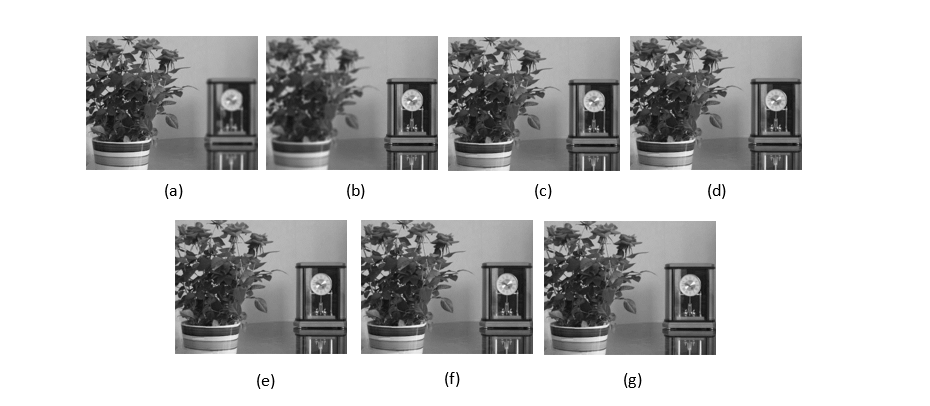
\includegraphics[width=0.9\textwidth]{fus1.png}
  \caption{Example of multifocus image fusion (a)(b) is source image (c)(d)(e)(f)(g) are fusion result for LP-SR, DWR-SR, DTCWT-ST, CVT-SR, NSCT-SR respectivley }\label{fus1}
\end{figure} 
The following table show the evaluation metrics for the above images is given in tabel\ref{tab1}

\begin{table}[!htb] 
 \centering
  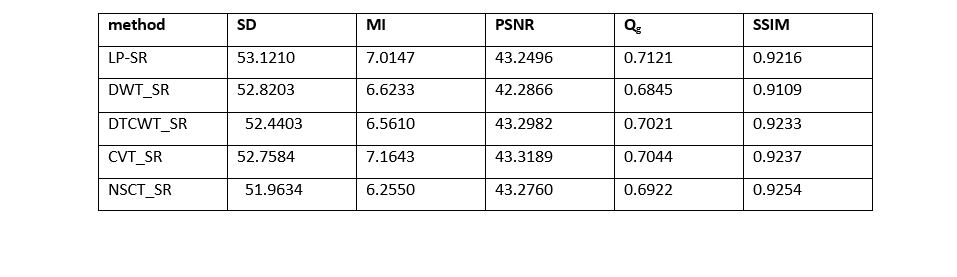
\includegraphics[width=.9\textwidth]{tab1.PNG}
  \caption{Evaluation metrics for different method}
  \label{tab1}
\end{table}

\begin{figure}[h!]
  \centering
  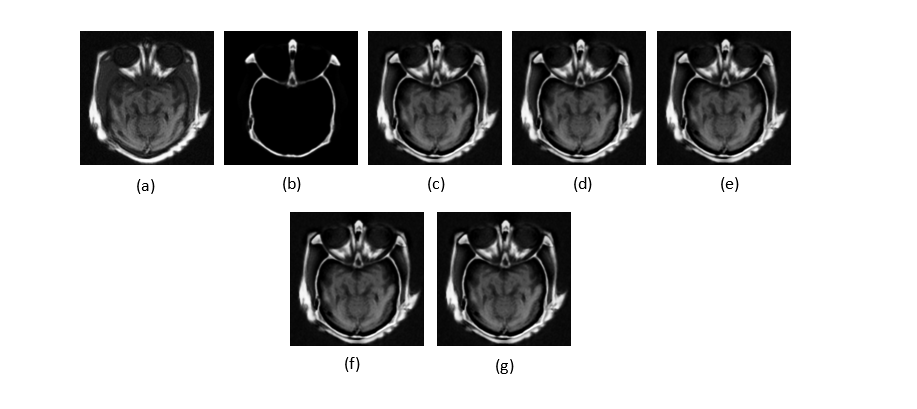
\includegraphics[width=.9\textwidth]{fus2.png}
  \caption{Example of  image fusion (a)MR(b)CT are source images (c)(d)(e)(f)(g) are fusion result for LP-SR, DWR-SR, DTCWT-ST, CVT-SR, NSCT-SR respectivley }\label{fus2}
\end{figure}

The evaluation metrics for different method for medical image is given in table\ref{tab2}

\begin{table}[!htb] 
 \centering
  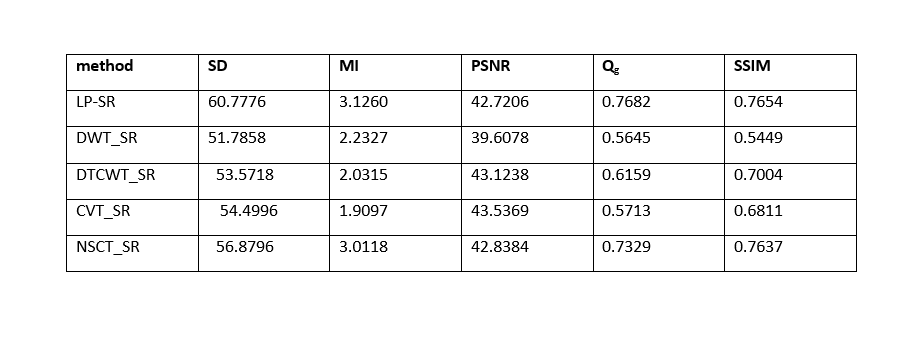
\includegraphics[width=.9\textwidth]{tab2.PNG}
  \caption{Evaluation metrics for different method for medical image}
  \label{tab2}
\end{table}

\begin{figure}[h!]
  \centering
  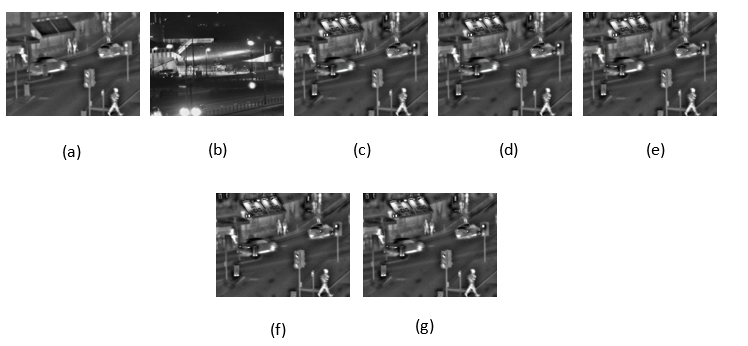
\includegraphics[width=.9\textwidth]{fus3.png}
  \caption{Example of  image fusion (a)infrared image(b)visible image are source images (c)(d)(e)(f)(g) are fusion result for LP-SR, DWR-SR, DTCWT-ST, CVT-SR, NSCT-SR respectivley }\label{fus3}
\end{figure}

The evaluation metrics for different method for visible infrared image is given in table\ref{tab3}

\begin{table}[!htb] 
 \centering
  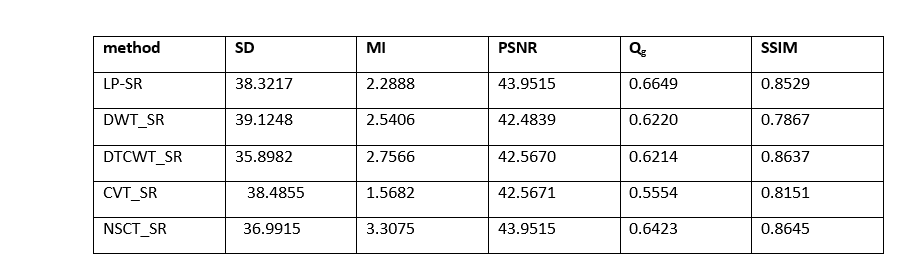
\includegraphics[width=.9\textwidth]{tab3.PNG}
  \caption{Evaluation metrics of different method for infrared image}
  \label{tab3}
\end{table}

Since now we give the experimental result that gives without the noise.When we add noise then how the \textbf{PSNR}  value varies with different values of \textbf{Sigma} is comparatively shown in fig\ref{graph1} for different \textbf{MST} method.I also put the value of psnr in Tabel.\ref{tab4} for multifocus image in Table\ref{tab5} for medical image and in Table\ref{tab6} for infrared image.  

\begin{table}[!htb] 
 \centering
  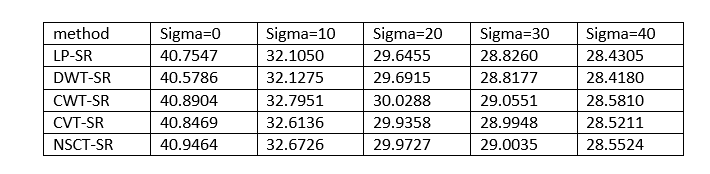
\includegraphics[width=.9\textwidth]{tab4.PNG}
  \caption{PSNR variation for different value of sigma for different method for multifocus image}
  \label{tab4}
\end{table}

\begin{figure}[h!]
  \centering
  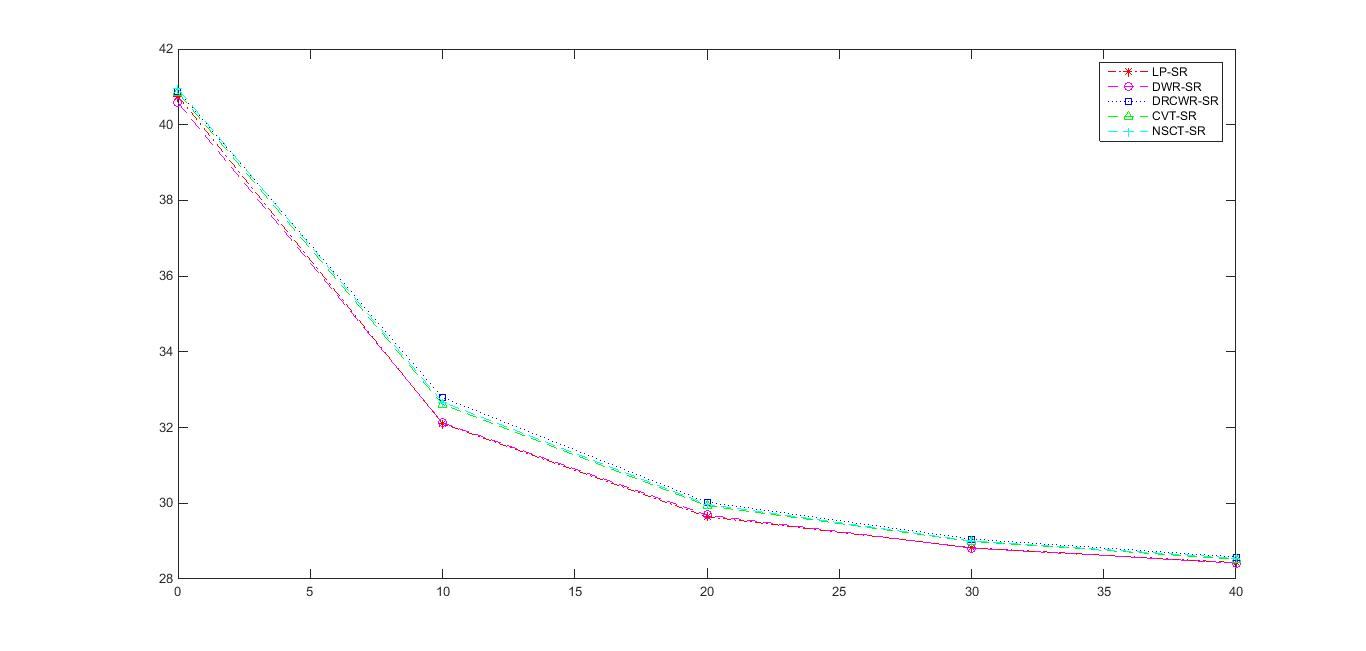
\includegraphics[width=.9\textwidth]{noisevar1.jpg}
  \caption{PSNR variation for different value of sigma for multifocus image of first image pair shown in figure \ref{fig:6.1}}\label{graph1}
\end{figure}

\begin{table}[!htb] 
 \centering
  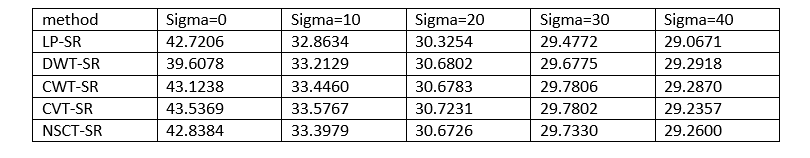
\includegraphics[width=.9\textwidth]{tab5.PNG}
  \caption{PSNR variation for different value of sigma for different method for medical image}
  \label{tab5}
\end{table}

\begin{figure}[h!]
  \centering
  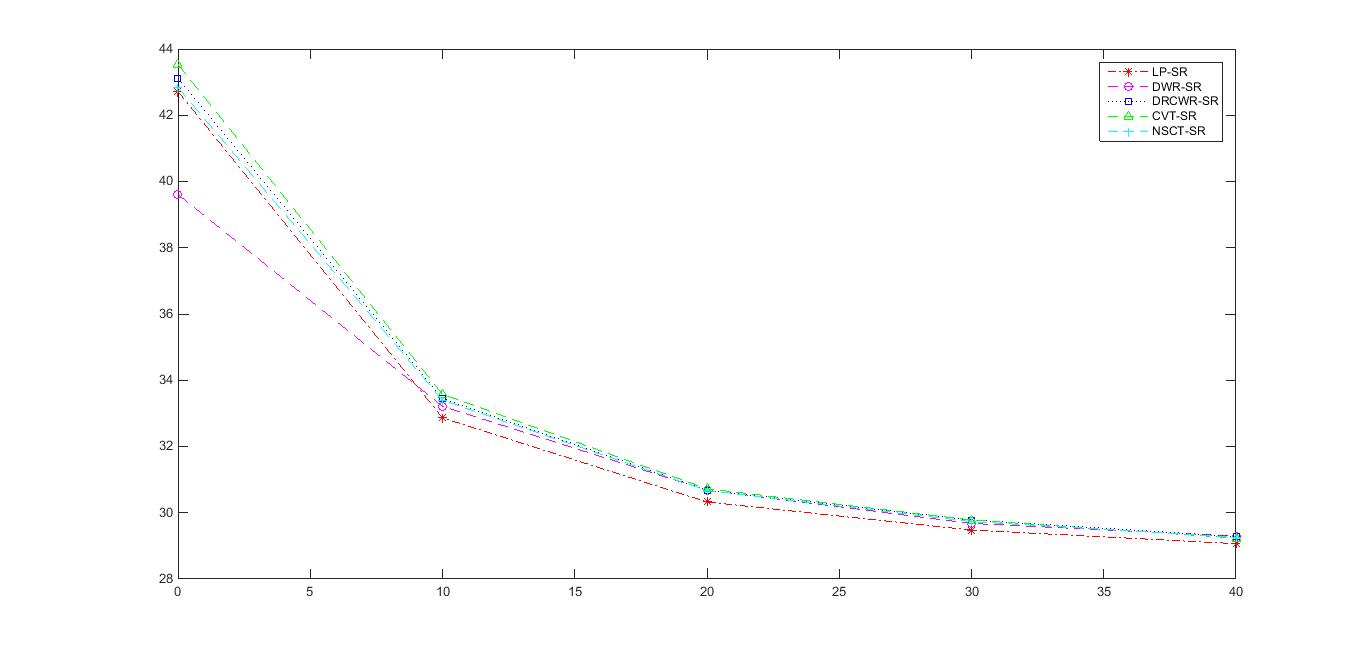
\includegraphics[width=.9\textwidth]{noisevar2.jpg}
  \caption{PSNR variation for different value of sigma for medical image of first medical image image pair shown in figure \ref{fig:6.1}}
  \label{graph2}
\end{figure}

\section{Discussion}
 for each type of image fusion, I take the related contents in Tables \ref{tab1}-\ref{tab5} into consideration together and seek out some common regularities among the six MST s used in the proposed framework. \hfill \break
 
 From the data obtained from table\ref{tab1}-\ref{tab5} and graph\ref{graph1}-\ref{graph2} we see that NSCT-SR based image fusion gives better result than other method.We perform this task on about 50 pair of image and this method gives the better result than any others method. 




\chapter{Conclusion and Future plan}
I proposed a general method for image fusion using MST and sparse representation.It gave us the result which overcome the disadvantage introduced in MST and SR method individually. Training time for Dictionary is relatively high.We use a dataset consisting different type of image and which contains about 40 images.For thresolding the image we use bayesShrik thresholding which take the threshold value in different direction of image under certain transformation domain, 
giving a good threshold result there for the image is noiseless in great measure. In the future, this model can be enhanced and cope
with different efficient transformation domain which can take the geometry of  image in better way. So it will be interesting to see how advancement is made in this approach.

%\chapter{The Architecture}
%\section{The Architecture}\label{sec:SysArchi}

\subsection{Architecture for tagging single label images}
In the figure \ref{singlelabel} is a cropped down version of the Convolutional Neural Network that is used to tag single label images. This has been given to give an idea about the network.

\begin{figure}[h!]
  \centering
  \includegraphics[width=.9\textwidth]{singlelabel.png}
  \caption{Convolutional Neural Network for tagging Single Label Images(Cropped Down)} \label{singlelabel}
\end{figure}

The full network is like the one in the figure. It has 59 layers in sequential manner. The input is the image and output is the label associated with that image.\hfill\break input\(\rightarrow\)1\(\rightarrow\)2\(\rightarrow\)3) \(\rightarrow\) (4) \(\rightarrow\) (5) \(\rightarrow\) (6) \(\rightarrow\) (7) \(\rightarrow\) (8) \(\rightarrow\) (9) \(\rightarrow\) (10) \(\rightarrow\) (11) \(\rightarrow\) (12) \(\rightarrow\) (13) \(\rightarrow\) (14) \(\rightarrow\) (15) \(\rightarrow\) (16) \(\rightarrow\) (17) \(\rightarrow\) (18) \(\rightarrow\) (19) \(\rightarrow\) (20) \(\rightarrow\) (21) \(\rightarrow\) (22) \(\rightarrow\) (23) \(\rightarrow\) (24) \(\rightarrow\) (25) \(\rightarrow\) (26) \(\rightarrow\) (27) \(\rightarrow\) (28) \(\rightarrow\) (29) \(\rightarrow\) (30) \(\rightarrow\) (31) \(\rightarrow\) (32) \(\rightarrow\) (33) \(\rightarrow\) (34) \(\rightarrow\) (35) \(\rightarrow\) (36) \(\rightarrow\) (37) \(\rightarrow\) (38) \(\rightarrow\) (39) \(\rightarrow\) (40) \(\rightarrow\) (41) \(\rightarrow\) (42) \(\rightarrow\) (43) \(\rightarrow\) (44) \(\rightarrow\) (45) \(\rightarrow\) (46) \(\rightarrow\) (47) \(\rightarrow\) (48) \(\rightarrow\) (49) \(\rightarrow\) (50) \(\rightarrow\) (51) \(\rightarrow\) (52) \(\rightarrow\) (53) \(\rightarrow\) (54) \(\rightarrow\) (55) \(\rightarrow\) (56) \(\rightarrow\) (57) \(\rightarrow\) (58) \(\rightarrow\) (59) \(\rightarrow\) output
\hfill\break
A short description about each layer is given below.\hfill\break (1): Spatial Convolution(3 \(\rightarrow\) 64, 3x3, 1,1, 1,1) \hfill\break
  (2): Spatial Batch Normalization \hfill\break
  (3): ReLU \hfill\break
  (4): Dropout(0.3) \hfill\break
  (5): Spatial Convolution(64 \(\rightarrow\) 64, 3x3, 1,1, 1,1) \hfill\break
  (6): Spatial Batch Normalization \hfill\break
  (7): ReLU \hfill\break
  (8): Spatial Max Pooling(2,2,2,2) \hfill\break
  (9): Spatial Convolution(64 \(\rightarrow\) 128, 3x3, 1,1, 1,1) \hfill\break
  (10): Spatial Batch Normalization \hfill\break
  (11): ReLU \hfill\break
  (12): Dropout(0.4) \hfill\break
  (13): Spatial Convolution(128 \(\rightarrow\) 128, 3x3, 1,1, 1,1) \hfill\break
  (14): Spatial Batch Normalization \hfill\break
  (15): ReLU \hfill\break
  (16): Spatial Max Pooling(2,2,2,2) \hfill\break
  (17): Spatial Convolution(128 \(\rightarrow\) 256, 3x3, 1,1, 1,1) \hfill\break
  (18): Spatial Batch Normalization \hfill\break
  (19): ReLU \hfill\break
  (20): Dropout(0.4) \hfill\break
  (21): Spatial Convolution(256 \(\rightarrow\) 256, 3x3, 1,1, 1,1) \hfill\break
  (22): Spatial Batch Normalization \hfill\break
  (23): ReLU \hfill\break
  (24): Dropout(0.4) \hfill\break
  (25): Spatial Convolution(256 \(\rightarrow\) 256, 3x3, 1,1, 1,1) \hfill\break
  (26): Spatial Batch Normalization \hfill\break
  (27): ReLU \hfill\break
  (28): Spatial Max Pooling(2,2,2,2) \hfill\break
  (29): Spatial Convolution(256 \(\rightarrow\) 512, 3x3, 1,1, 1,1) \hfill\break
  (30): Spatial Batch Normalization \hfill\break
  (31): ReLU \hfill\break
  (32): Dropout(0.4) \hfill\break
  (33): Spatial Convolution(512 \(\rightarrow\) 512, 3x3, 1,1, 1,1) \hfill\break
  (34): Spatial Batch Normalization \hfill\break
  (35): ReLU \hfill\break
  (36): Dropout(0.4) \hfill\break
  (37): Spatial Convolution(512 \(\rightarrow\) 512, 3x3, 1,1, 1,1) \hfill\break
  (38): Spatial Batch Normalization \hfill\break
  (39): ReLU \hfill\break
  (40): Spatial Max Pooling(2,2,2,2) \hfill\break
  (41): Spatial Convolution(512 \(\rightarrow\) 512, 3x3, 1,1, 1,1) \hfill\break
  (42): Spatial Batch Normalization \hfill\break
  (43): ReLU \hfill\break
  (44): Dropout(0.4) \hfill\break
  (45): Spatial Convolution(512 \(\rightarrow\) 512, 3x3, 1,1, 1,1) \hfill\break
  (46): Spatial Batch Normalization \hfill\break
  (47): ReLU \hfill\break
  (48): Dropout(0.4) \hfill\break
  (49): Spatial Convolution(512 \(\rightarrow\) 512, 3x3, 1,1, 1,1) \hfill\break
  (50): Spatial Batch Normalization \hfill\break
  (51): ReLU \hfill\break
  (52): Spatial Max Pooling(2,2,2,2) \hfill\break
  (53): View \hfill\break
  (54): Dropout(0.5) \hfill\break
  (55): Linear(512 \(\rightarrow\) 512) \hfill\break
  (56): Batch Normalization \hfill\break
  (57): ReLU \hfill\break
  (58): Dropout(0.5) \hfill\break
  (59): Linear(512 \(\rightarrow\) 10) \hfill\break
  
  
  \paragraph{Spatial Convolution:}
  
  Applies a 2D convolution over an input image composed of several input planes. For an example, Spatial Convolution(3 \(\rightarrow\) 64, 3x3, 1,1, 1,1) means that number of input channel is 3, and the number of output channel is 64. The kernel size is 3x3 and as there are 64 output channels, there will be 64 kernels, each having dimension 3x3. The step of the convolution is 1 step for height and width. The padding is 1 for height and width. Let's visualize this. In the figure \ref{spatialconv} the input neurons are the ones representing each pixel of an image, the kernel size or the filter size is 5x5. This filter would iterate over every single pixel and for each pixel look at the 5x5 neighborhood and produce corresponding images. As the number of output channel is 64, this will be done 64 times.
  
  \begin{figure}[h!]
  \centering
  \includegraphics[width=.9\textwidth]{spatialconv.png}
  \caption{Spatial Convolution with Kernel Size 5x5} \label{spatialconv}
\end{figure}

\paragraph{Spatial Batch Normalization:}

Implements Batch Normalization as described in the paper \cite{6}. The operation implemented is:

 $$y=\frac{x - mean(x)}{standard \textendash deviation(x)} * gamma + beta$$
 
 where the mean and standard-deviation are calculated per feature-map over the mini-batches and pixels and where gamma and beta are learnable parameter vectors of size N (where N = number of feature maps).
 
 
 \paragraph{ReLU:}
 It is the activation function defined as: $$f(x) = max(0,x)$$.
 
 
 \paragraph{Spatial Max Pooling:}
 Applies 2D max-pooling operation. For example, Spatial Max Pooling(2,2,2,2) means that the max pooling will be done with filter 2x2 with step 2 in height and step 2 in width direction. Max pooling means that we will select the maximum value from 2x2 filter or the input area.
 
 
 \paragraph{Dropout:}
 Dropout is used to prevent the neural network from overfitting. Dropout is implemented by only keeping a neuron active with some probability p (a hyperparameter), or setting it to zero otherwise. The input neuron is scaled by $1/p$ if it is not deactivated.
 
 \paragraph{Linear:}
 Applies a linear transformation to the incoming data ($y = mx + c$). For example, Linear(512 \(\rightarrow\) 10) means that there are 512 input channels and these 512 channels are converted to 10 channels. So, the weight matrix will be 10x512. 
 
 
 \paragraph{Loss Function:}
 Cross-entropy loss function has been used which has the form:
 
 
$$ L_{i} = -\log{(\frac{e^{f_y}}{\sum_j{e^{f_j}}})}$$

\subsection{Normalization on CIFAR-10}

Normalization is required so that all the inputs are at a comparable range. This can be done to force the input values to a certain range. The images were converted from RGB channel to YUV channel. Then U and V channels were normalized globally with mean and standard deviation. The Y channel was normalized locally.

\section{Object Recognition}
There are many approaches for segmenting an image having multiple objects into many segmented images. Our target is to take any approach and pass it to our trained CNN model. We found out two established approaches and tried on that.

\subsection{Measuring the objectness of image windows}
B. Alexe et al. \cite{1} presented a generic objectness measure, quantifying how likely it is for an image window to contain an object of any
class. They explicitly trained it to distinguish objects with a well-defined boundary in space, such as cows and telephones, from amorphous
background elements, such as grass and road. The measure combines in a Bayesian framework several image cues measuring
characteristics of objects, such as appearing different from their surroundings and having a closed boundary. These include an
innovative cue to measure the closed boundary characteristic. Finally, they presented two applications of objectness. In the first, they sample a small number windows according to their
objectness probability and gave an algorithm to employ them as location priors for modern class-specific object detectors. As they showed

\begin{figure}[ht] 
  \begin{subfigure}[b]{0.5\linewidth}
    \centering
    \includegraphics[width=0.9\linewidth]{obj1}
    \caption{} 
    \label{obj1} 
    \vspace{4ex}
  \end{subfigure}%%
  \begin{subfigure}[b]{0.5\linewidth}
    \centering
    \includegraphics[width=0.9\linewidth]{obj2}
    \caption{} 
    \label{obj2} 
    \vspace{4ex}
  \end{subfigure}%%
  \caption{Segmented Images}
  \label{objectnessfig} 
\end{figure}

experimentally, this greatly reduces the number of windows evaluated by the expensive class-specific model. In the second application,
they used objectness as a complementary score in addition to the class-specific model, which leads to fewer false positives. As shown in
several recent papers, objectness can act as a valuable focus of attention mechanism in many other applications operating on image
windows, including weakly supervised learning of object categories, unsupervised pixelwise segmentation, and object tracking in video.
Computing objectness is very efficient and takes only about 4 sec. per image. This technique finds out some image windows like Figure \ref{objectnessfig}. \hfill \break

\begin{algorithm}[H]
\SetAlgoLined
\begin{description}\itemsep1pt \parskip0pt \parsep0pt \vspace{.5cm}
  \item[Input:] \(F, D, c\) 
  \item[Ouput:] \(Det\)
  \item[Step 1:] \( \l = \left \{ w_{1},...,w_{F} \right \}, w_{i}\rightarrow D, \forall_{i} \)
  \item[Step 2:] \( \l_{s} = \left \{ \left ( w_{1},sw_{1} \right ),...,\left ( w_{F},sw_{F} \right )  \right \}, sw_{i}= c\left ( w_{i} \right ), \forall_{i} \) 
  \item[Step 3:] \( \rho _{s} = NMS\left ( \l_{s} \right )=\left \{ \left ( w_{n1},sw_{n1} \right ),...,\left ( w_{np},sw_{np} \right )  \right \}\)
  \item[Step 4:] \(\L=\left \{ w_{n1}^{lm},..., w_{np}^{lm} \right \}, w_{nj}^{lm} = max \left ( s_{w} \right )\)
  \item[Step 5:] \(Det = NMS\left ( \L \right )\)
\end{description}
\caption{Using objectness for class-specific detectors.}
\end{algorithm}

\hfill \break
The general scheme for using their objectness measure as
a location prior for object detectors is algorithm 1. The
algorithm inputs the class-specific confidence function \(c\) which
the detector employs to score a window.
They build an initial set \(\l\) of \(F = 1000\) windows multinomially sampled from the distribution \(D\) of windows scored by
their objectness measure (Multi-scale Saliency)\(MS\) +(Color Contrast)\(CC\) + (Superpixels Straddling)\(SS\) (step 1). They use \(c\) to
score each window in \(\l\) (step 2). They then run the non-maxima
suppression. This results in a set \(\rho_{s}\) of promising
windows (step 3). For every window \(w_{p} \epsilon \rho_{s}\), they iteratively
move to the local maximum of \(c\) in its neighborhood \(V_{w
p}\),
resulting in window \(w_{p}^{lm}\) (step 4). Finally, they run \(NMS\) on the
local maxima windows \(\L\) and obtain detections \(Det\) (step 5).
In order to use this algorithm one has to specify a window
scoring function \(c\), which is specific to a particular detector
and object class, and a window neighborhood.



\subsection{Selective Search for Object Recognition}

%\begin{algorithm}[H]
%\SetAlgoLined
%\KwData{(color) image}
%\KwResult{Set of object location hypotheses \(L\) }\break
% Obtain initial regions \(R = \left \{ r_{1},..., r_{n} \right \}\) using [13]\break
% Initialize similarity set \(S = \varnothing\)
% \foreach{abc}
% \While{While condition}{
%  instructions\;
%  \eIf{condition}{
%   instructions1\;
%   instructions2\;
%   }{
%   instructions3\;
%  }
% }
% \caption{How to write algorithms}
%\end{algorithm}

J.R.R. Uijlings et al. \cite{2} took a hierarchical grouping algorithm to form the basis of their
selective search. Bottom-up grouping is a popular approach to segmentation, hence they adapted it for selective search. Because
the process of grouping itself is hierarchical, they can naturally generate locations at all scales by continuing the grouping process until
the whole image becomes a single region. This satisfies the condition of capturing all scales.
As regions can yield richer information than pixels, they wanted to
use region-based features whenever possible. To get a set of small
starting regions which ideally do not span multiple objects, they used the fast method of Felzenszwalb and Huttenlocher \cite{7}, which
found well-suited for such purpose.
Their grouping procedure now works as follows. They first used \cite{7}
to create initial regions. Then they used a greedy algorithm to iteratively group regions together: First the similarities between all
neighbouring regions are calculated. The two most similar regions
are grouped together, and new similarities are calculated between
the resulting region and its neighbours. The process of grouping
the most similar regions is repeated until the whole image becomes
a single region.


\section{Architecture For tagging Multi-Label Images}

Our Final architecture for tagging multi-label images consists of (1) image segmentation and (2) convolutional neural network for detecting segmented images. The image segmentation techniques, objectness measures and selective search and the architecture for single label image detection has been described before. In the Figure \ref{finalarch} there is an overview of the architecture. \hfill \break

\begin{figure}[h!]
  \centering
  \includegraphics[width=0.9\textwidth]{finalarch.png}
  \caption{Architecture of Tagging Multi-Label Images}\label{finalarch}
\end{figure}

At first we segment the image with objectness measures and selective search. Then we get multiple segmented images. Note that there will be many segment images. In the figure only a few are shown. Then we pass the segmented images through the convolutional neural network that tags the label associated with that image. As there are many segmented images, there may be some labels that will be wrongly tagged. We inspect these labels and their associative scores and finally conclude which of the labels are likely to be associated with the images. We performed several techniques for inspecting the images. These are discussed in the experimental result section.



%\chapter{Proposed Algorithm}
%\section{The ADC-QSIN algorithm for scheduling multi-item queries using network coding} 

%\chapter{Experimental Result}
%\section{Experimental Result for CIFAR-10}

In the Table \ref{cifar10conf} there is the result for the testing images of CIFAR-10 dataset. Here, each row represents the testing label, each column represents the label produced by the network. For example the cell (1,1) represents that the testing label is airplane and the tagged label is airplane, the cell (1,2) represents that the testing label is airplane and the tagged label is automobile. So, each cell (i,i) where $[i = 1..10]$ represents the correctly tagged labels. Each row consists of 1000 image labels. So the accuracy will be cell$(i,i)/1000$.

%\begin{figure}[h!]
%  \centering
%  \includegraphics[width=0.9\textwidth]{cifar10.PNG}
%  \caption{CIFAR-10 Confusion Matrix}\label{cifar10conf}
%\end{figure}


\begin{table}[!htb] 
 \centering
  \includegraphics[width=0.9\textwidth]{cifar10.PNG}
  \caption{CIFAR-10 Confusion Matrix}
  \label{cifar10conf}
\end{table}


\section{Experimental Result for Multi-Label Image tagging}
To give an overview of the process of inspecting the result of the segmented images, we will need the help of Table \ref{score}. The table is for a single multi-label image. Each $image_{i}$ represents the segmented image from the multi-label image. Each row represents the class scores given by the network. 

\paragraph{Selecting Top-1 Score:}
In this approach we select the top 1 score and its associating label from each segmented image $image_{i}$. Then we increase the frequency of labels for each top 1 score. After that we select the top 4 scoring labels. For example, in the Table \ref{score} the top 1 label for $image_{1}$ would be cat. So we increase the frequency of cat by 1. Similarly for $image_{2}$ again the score for label cat is highest. So frequency of cat will be increased by 1.

%\begin{figure}[h!]
%  \centering
%  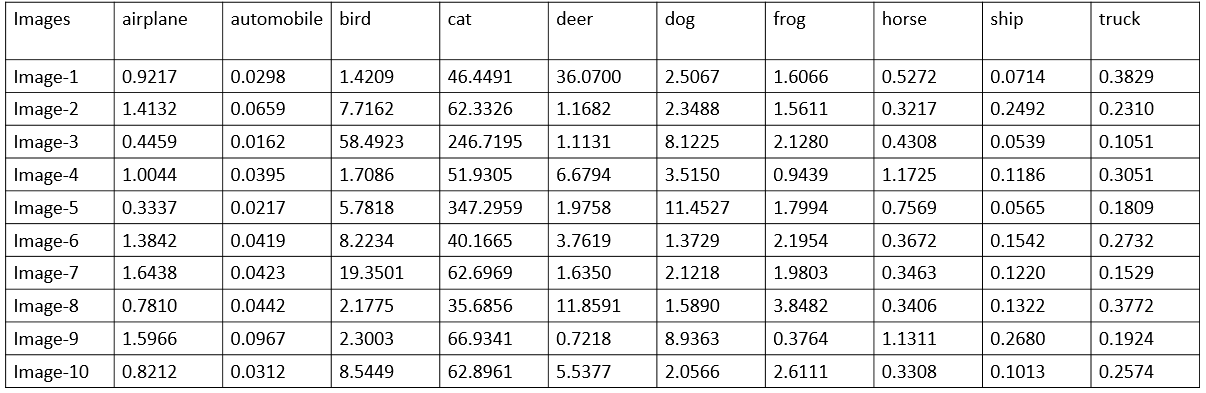
\includegraphics[width=0.9\textwidth]{newresult.PNG}
%  \caption{Scores for the sample image}\label{score}
%\end{figure}

\begin{table}[!htb]
 \centering
  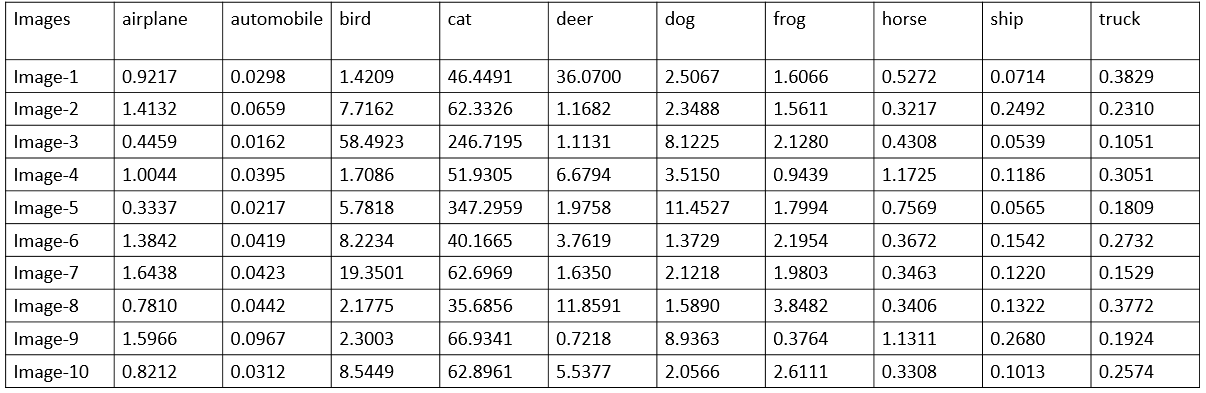
\includegraphics[width=0.9\textwidth]{newresult.PNG}
  \caption{Scores for the sample image}
  \label{score}
\end{table}

\paragraph{Selecting Top-2 Score:}
In this approach we select the top 2 scores and its associating label from each segmented image $image_{i}$. Then we increase the frequency of labels for each top 2 scores. After that we select the top 4 scoring labels.  For example, in the Table \ref{score} the top 2 labels for $image_{1}$ would be cat and deer. So the frequency of cat and deer will be increased by 1.

%\begin{figure}[h!]
%  \centering
%  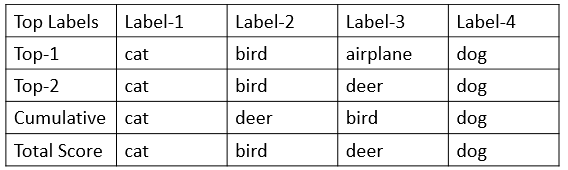
\includegraphics[width=0.9\textwidth]{result_objectness.PNG}
%  \caption{Result for the sample image for Objectness Measures}\label{resobj}
%\end{figure}

\begin{table}[!htb]
\centering
  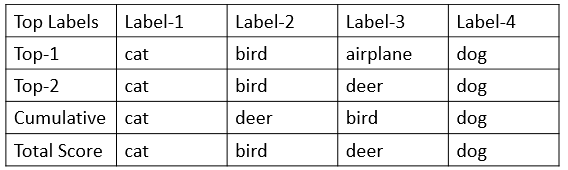
\includegraphics[width=0.9\textwidth]{result_objectness.PNG}
  \caption{Result for the sample image for Objectness Measures}
   \label{resobj}
\end{table}

\paragraph{Selecting Total Score:}
In this approach we just add all scores of each $label_{i}$ for each segmented image $image_{i}$. Then we select the top 4 scoring labels. For example, every class score for every label will be added. So, the score for cat label will be the total score in the column cat. Similarly the score for bird will be the total score in the column bird.

%\begin{figure}[h!]
%  \centering
%  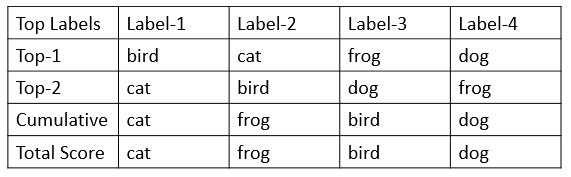
\includegraphics[width=0.9\textwidth]{result_selective.PNG}
%  \caption{Result for the sample image for Selective Search}\label{ressel}
%\end{figure}

\begin{table}[!htb]
\centering
  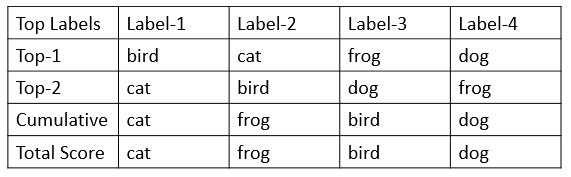
\includegraphics[width=0.9\textwidth]{result_selective.PNG}
  \caption{Result for the sample image for Selective Search}
  \label{ressel}
\end{table}

\paragraph{Selecting Cumulative Percentage:}
Each $label_{i}$ of segmented image $image_{i}$ has the percentage $score_{i} / \sum_{i}{score_{i}}$. We select the top percentage from each segmented image $image_{i}$. We add these percentages for each associated labels and select the top 4 scoring labels. For example for $image_{1}$ the percentage of cat will be $score_{cat} / \sum_{i}{score_{i}}$.\hfill \break

The results for these four approaches for the sample image from Figure \ref{sample_multi_label} is given at Table \ref{resobj} and Table \ref{ressel} \hfill \break


These approaches were repeated in our selected multi label images. The results for Objectness Measure is given in Figure \ref{finobj} and for Selective Search in Figure  \ref{finsel}

\begin{figure}[h!]
  \centering
  \includegraphics[width=0.5\textwidth]{sample_multi_label.PNG}
  \caption{Sample Multi-Label Image}\label{sample_multi_label}
\end{figure}


\begin{figure}[h!]
  \centering
  \includegraphics[width=0.5\textwidth]{Capture3.PNG}
  \caption{Result for multi-label images for Objectness Measures}\label{finobj}
\end{figure}


\begin{figure}[h!]
  \centering
  \includegraphics[width=0.5\textwidth]{Capture4.PNG}
  \caption {Result for multi-label images for Selective Search}\label{finsel}
\end{figure}

\section{Discussion}

The main problem of tagging multi-label images are the training time required. If Convolutional Neural Network is used for tagging multiple labels, then there is a chance that the networks will be very complex. This will require a lot of time to train. Also, if it takes a lot of time to train, then tweaking the network and exploring promising functionalities will require a lot of time. But our Convolutional Neural Network can only tag Single Label images, then we use this network to tag the segmented images provided by Objectness Measures and Selective Search approach. The Convolutional Neural Network we provided is faster to train, so tweaking the network will provide quick result. We got about 57\% accuracy using the Selective Search approach shown in \ref{finsel}. So, we can expect that if we increase the capability of our network, this accuracy will be much higher.



%\chapter{Tools and Recommendations for Future Works}
%\section{Used Tools}
\subsubsection{Torch}
Torch is a scientific computing framework with wide support for machine learning algorithms. It is easy to use and efficient. At the heart of Torch are the popular neural network and optimization libraries which are simple to use, while having maximum flexibility in implementing complex neural network topologies.\hfill \break 

Our Convolutional Neural Network runs on top of Torch.

\subsubsection{Waffle}
Waffle is a fast, asynchronous, express-inspired web framework for Torch built on top of ASyNC. \hfill \break

We used this to build a server that tags the single and multi-label images.

\section{Future Works}
The strength of our multi-label image tagging architecture depends on convolutional neural network classifier and the method for segmenting images.\hfill \break

So, be refining out convolutional neural network to include more labels by training CIFAR-100 and using better methods to segment the image, we can improve the performance of the network.\hfill \break

As the image segmentation techniques give duplicate segmented images, so to sort out all the unique segmented images can be a nice challenge to achieve.

%\chapter{Conclusion}
%We have presented an easy and simple approach to tag multi-label images using a trained CNN classifier with objectness measure and selective search of an image. It gave us the result in quick time. Our training time for CNN network is fast. Segmenting the images is also fast. Our technique is a stepping stone to this approach. It is giving a good threshold result. In the future, this model can be enhanced and cope with larger dataset. So it will be interesting to see how advancement is made in this approach.


%\appendix
%\chapter{Appendix}
%\input{chapters/appendix}

\begin{thebibliography}{150}

    % Set Reference ID carefully, do not use replication
    
   \bibitem {1}P. Burt, E. Adelson, The laplacian pyramid as a compact image code, IEEE Trans.Commun. 31 (4) (1983) 532–540..
 
 \bibitem {2} P. Burt, E. Adelson, The laplacian pyramid as a compact image code, IEEE Trans.Commun. 31 (4) (1983) 532–540
 

\bibitem {3} A. Toet, Image fusion by a ratio of low pass pyramid, Pattern Recogn. Lett. 9(4)(1989) 245–253.

\bibitem {4} V. Petrovic, C. Xydeas, Gradient-based multiresolution image fusion, IEEE Trans. Image Process. 13 (2) (2004) 228–237.


\bibitem {5} H. Li, B. Manjunath, S. Mitra, Multisensor image fusion using the wavelet transform, Graph. Models Image Process. 57 (3) (1995) 235–245


\bibitem{6} M. Beaulieu, S. Foucher, L. Gagnon, Multi-spectral image resolution refinement using stationary wavelet transform, in: Proceedings of 3rd IEEE International Geoscience and Remote Sensing Symposium, 2003, pp. 4032–4034


\bibitem{7}J. Lewis, R. OCallaghan, S. Nikolov, D. Bull, N. Canagarajah, Pixel- and regionbased image fusion with complex wavelets, Inform. Fusion 8 (2) (2007) 119–130.

\bibitem{8} F. Nencini, A. Garzelli, S. Baronti, L. Alparone, Remote sensing image fusion using the curvelet transform, Inform. Fusion 8 (2) (2007) 143–156

\bibitem{9}M. Aharon, M. Elad, and A. Bruckstein,“K-SVD: an algorithm for designing overcomplete dictionaries for sparse representation,”IEEE Trans. Signal Process.54(11), 4311–4322(2006)

\bibitem{10}T. Guha and R. K. Ward,“Learning sparse representations for human action recognition,” IEEE Trans. Pattern Anal. Mach. Intell 34(8),1576–1588 (2012)

\bibitem{11}M. S. Lewicki and T. J. Sejnowski,“Learning overcomplete representations,”Neural Comput.12(2), 337–365 (2000)

\bibitem{12}K. Engan, S. O. Aase, and J. H. Husoy,“Method of optimal directions for frame design,”in Int. Conf. Audio, Speech and Signal Processing, Vol. 5, pp. 2443–2446, IEEE Press, Phoenix, AZ (1999).

\bibitem{13} M. Yaghoobi, T. Blumensath, and M. E. Davies,“Dictionary learning for sparse approximations with the majorization method,”IEEE Trans. Signal Process.57(6), 2178–2191 (2009)

\bibitem{14} L. Landweber,“An iterative formula for fredholm integral equations of the first kind,”Am. J. Math.73(3), 615–624 (1951)

\bibitem{15}B. Yang and S. Li,“Multifocus image fusion and restoration with sparse representation,”IEEE Trans. Instrum. Meas. 59(4), 884–892 (2010).

\bibitem{16}B. A. Olshausen and D. J. Field, “Emergence of simple-cell receptive field properties by learning a sparse coding for natural images,”Nature, vol. 381, no. 6583, pp. 607–609, Jun. 1996

\bibitem{17}G. Davis, S. Mallat, and M. Avellaneda, “Adaptive greedy approximations,”Constr. Approx., vol. 13, no. 1, pp. 57–98, Mar. 1997.

\bibitem{18} M. Aharon, M. Elad, and A. Bruckstein, “K-SVD: An algorithm for designing overcomplete dictionaries for sparse representation,”IEEE Trans.Signal Process., vol. 54, no. 11, pp. 4311–4322, Nov. 2006.

\bibitem{19}I. F. Gorodnitsky and B. D. Rao, “Sparse signal reconstruction from limited data using FOCUSS: A re-weighted norm minimization algorithm,”IEEE Trans. Signal Process., vol. 45, no. 3, pp. 600–616, Mar. 1997.

\bibitem{20}M. Elad and M. Aharon, “Image denoising via sparse and redundant representations over learned dictionaries,” IEEE Trans. Image Process.,vol. 15, no. 2, pp. 3736–3745, Dec. 2006.

\bibitem{21}Iain M.Johnstone David L Donoho. Adapting to smoothness via wavelet shrinkage.Journal of the Statistical Association, 90(432):1200–1224, Dec 1995.

\bibitem{22} David L Donoho. Ideal spatial adaptation by wavelet shrinkage. Biometrika,

\bibitem{23} David L Donoho. De-noising by soft thresholding. IEEE Transactions on Information Theory, 41(3):613–627, May 1995.

\bibitem{24}S. Mallat, Z. Zhang, Matching pursuits with time-frequency dictionaries, IEEE Trans. Signal Process. 41 (12) (1993) 3397–3415.

\bibitem{25}S. Li, B. Yang, J. Hu, Performance comparison of different multi-resolution transforms for image fusion, Inform. Fusion 12 (2) (2011) 74–84.

\end{thebibliography}


\end{document}
